\documentclass[a4paper,12pt,twoside]{report} % font size 12 linespace 1.5
\usepackage[toc,page]{appendix}


%\documentclass[10pt,a4paper]{article}
%\usepackage{luatextra}                                                      
%\usepackage{fontspec}
%\setmainfont[BoldFont = Yu Mincho Demibold ]{Yu Mincho Medium}



\usepackage{tensor}
\usepackage{hyperref}
\usepackage{booktabs}
\usepackage{cancel}
%\usepackage{amsthm}
%\usepackage[utf8]{inputenc}

%\documentclass[11pt,a4paper,twoside]{report}
%\usepackage[english]{babel}

%\def\division{\char'057}
%\setlength{\unitlength}{.95pt}
%\renewcommand{\baselinestretch}{1.3}

\usepackage{setspace}
\onehalfspacing
\usepackage{ae,aecompl}
\usepackage[latin1]{inputenc}
\usepackage{graphicx}
\usepackage{bm}
\usepackage{amsmath,amssymb}
\DeclareSymbolFontAlphabet{\amsmathbb}{AMSb}
\usepackage{braket}
\usepackage{bbold}
\usepackage{tikz}
\usetikzlibrary{decorations.pathmorphing}
\usetikzlibrary{positioning}
%\font\sansserif=cmss10
%\renewcommand{\baselinestretch}{1.2}
%\setlength{\textwidth}{15cm}
%\setlength{\textheight}{29.7cm}
%\setlength{\topskip}{0cm}
%\setlength{\footskip}{0cm}
%\addtolength{\oddsidemargin}{-2cm}
%\addtolength{\topmargin}{-5cm}

\setlength\parindent{0pt}
\setlength\parskip{5pt}
\usepackage[top = 3cm, bottom = 3cm, inner = 4cm, outer = 1.7cm]{geometry}
 %\geometry{
% a4paper,
% %total={170mm,257mm},
% left=25mm,
% right=25mm,
% top=25mm,
% bottom = 35mm,
% }




%\theoremstyle{definition}
%\newtheorem{definition}{Definition}[section]

\newenvironment{proof}[1][Proof]{\begin{trivlist}
\item[\hskip \labelsep {\bfseries #1}]}{\end{trivlist}}
\newenvironment{definition}[1][Definition]{\begin{trivlist}
\item[\hskip \labelsep {\bfseries #1}]}{\end{trivlist}}
\newenvironment{example}[1][Example]{\begin{trivlist}
\item[\hskip \labelsep {\bfseries #1}]}{\end{trivlist}}
\newenvironment{remark}[1][Remark]{\begin{trivlist}
\item[\hskip \labelsep {\bfseries #1}]}{\end{trivlist}}



\newcommand{\op}[1]{\hat{\mathcal{{#1}}}}



\begin{document}
\begin{titlepage}
\setcounter{page}{1}

\begin{center}

\vspace*{3cm}
%\special{psfile="vaakuna.eps" vscale=22 hscale=22 voffset=-150 hoffset=127}
%\special{psfile="vaakuna.eps" width=0.5\textwidth}
\includegraphics[width=45mm]{Title/vaakuna.eps}

\vspace*{2cm}

Master's Thesis - Theoretical Physics \\
%(koulutusohjelma tähän)

\vspace{2.0cm} 
{\Large \bf
  \rule{0pt}{3ex}{Semi-Classical Conformal Blocks in the AdS/CFT correspondence and Their Applications}
}

\title{
 (%otsikko tähän)
}
%\maketitle

\vspace{2.0cm} 
Anshuman Dubey\\
2016

\vspace{1.5cm} 
\begin{tabular}{ll}	Advisor: & 	Esko Keski-Vakkuri \\ 
			Examiners: &	Kari Rummukainen \\
				     &	Esko Keski-Vakkuri
\end{tabular}

\vspace{1.5cm} University of Helsinki

Department of Physics

%\vspace{0.5cm} PL 64 (%Gustaf Hällströmin katu 2)

%00014 Helsingin yliopisto

\end{center}

\end{titlepage}

%\chapter*{Abstract}
Conformal blocks are building blocks of correlation functions in conformal field theories. They neatly encode the universal information dictated by conformal symmetry and separate it from the dynamical information which depends on the particular theory. Conformal blocks merit an in-depth study as is evidenced by their extensive applications in the study of bulk locality in the AdS/CFT correspondence and the recent Conformal Bootstrap program. The vacuum Virasoro blocks in the semi-classical (large central charge) limit is known to compute the leading order contribution to the R\'{e}nyi entropy. Moreover, the semi-classical Virasoro blocks along with conformal bootstrap feature in a proof of the cluster decomposition principle for AdS$_3$/CFT$_2$. 


Conformal field theory and its necessary ingredients are briefly reviewed. 3D gravity including its Chern-Simons formulation are briefly introduced. Conformal blocks from the exchange of a spinless operator are evaluated by holographic computations of geodesic Witten diagrams for AdS$_{n+1}$/CFT$_n$. The results are verified against the Casimir operator method of Dolan and Osborn. The procedure is extended to exchange of a spinning operator. Virasoro blocks in various semi-classical limits are discussed and connection is made with the Chern-Simons formulation of 3D gravity. Expressions for perturbative scalar (corresponding to exchange of spinless operator) Virasoro blocks are calculated in the global and heavy-light limit using the holographic approach. The results are extended to Virasoro blocks for the exchange spinning operators, and the results are verified using the monodromy method.


The Virasoro blocks thus obtained are used to calculate the two interval R\'{e}nyi entropy. A brief introduction is presented to the Conformal Bootstrap, followed by explicit derivation of the Cluster Decomposition principle for AdS$_3$/CFT$_2$.




\iffalse
The focus in the first part is on providing the relevent background. Starting with an introduction to the necessary ingredients from conformal field theory, including Zomolodchokov's recursion relations. Mellin representations of conformal correlation functions and Witten diagrams are discussed. Virasoro blocks are discussed in the different semi-classical limits. Perturbative Virasoro blocks corresponding to the exchange of a spin-less operator are computed in the heavy-light and global limits. The results are extended to Virasoro blocks arising from the exchange of an operator carrying spin. The calculations are done using AdS$_3$/CFT$_2$ holographic computations. For the heavy-light limit, the idea is calculating geodesic Witten diagrams for the light operators interacting in a background created by letting the heavy operators backreact. The geometry thus obtained can be either a BTZ black hole or a conical defect in AdS$_3$.

Lastly, applications to calculating two interval R\'{e}nyi entropy are discussed. Also, using the Conformal Bootstrap to constrain operator dimensions in CFTs is briefly introduced.
\fi
\tableofcontents
%\tableofcontents
\newpage
  \chapter{Introduction}
  \subsection{Motivation}
  \subsection{Current progress}
  \subsection{Objective}
  \section{Conformal Field Theory and Conformal Blocks}
  \subsection{Review of Conformal Field Theory}
  \subsection{4-Point Correlators and Block Decomposition}
  \subsection{Recursion Relations}
  \subsection{Integral Representations}
  \section{Introduction to 2+1 Gravity}
  \subsection{Review}
  \subsection{BTZ black holes and Conical Defects}
  \subsection{Chern-Simons formulation}
  \section{Mellin Space Technology}
  \subsection{AdS/CFT Considerations and Witten Diagrams}
  \subsection{Mellin Space Representations of CFT Correlators}
  \subsection{Mellin Amplitudes for Witten Diagrams}
  \section{Virasoro Blocks and the Semi-Classical Limit}
  \subsection{Introduction}
  \subsection{Spectrum of Semi-Classical Limits}
  \subsubsection{Global Limit}
  \subsubsection{Heavy-Light Limit}
  \subsubsection{Perturbative Heavy Limit}
  \subsubsection{Non-Perturbative Heavy Limit}
  \subsection{Operator Exchange: Spinless vs Spinning}
  %\subsection{Mellin Space Technology}
  \subsection{Monodromy Method and Liouville Theory}
  \subsection{Holographic Computation}
  \section{Applications}
  \subsection{R\'enyi Entropy}
  \section{Conclusions and Discussion}

\chapter{Introduction}
\section{Motivation}
\section{Current Progress}
\section{Objective}

\chapter{Conformal Field Theory and Conformal Blocks}

The ubiquitous nature of conformal field theories in Theoretical and Mathematical physics has lead to their extensive study in the past years. Conformal field theories describe worldsheet dynamics in string theory, describe statistical systems at points of second order phase transitions and appear as renormalization group fixed points of quantum field theories.

A conformal field theory is a quantum field theory that is invariant under local conformal transformations. Conformal transformations are the transformations that preserve angles, but not necessarily lengths. The Lorentz transformations naturally preserve angles between spacetime vectors and thus form a subset of conformal transformations, therefore, the Lorentz group is a subgroup of the conformal group. The particle states in the theory then fit in irreducible representations of the conformal group. Since conformal invariance implies scale invariance the particle excitations in the theory have to be massless. This section gives a brief review of the general properties of conformal field theory.

  \section{Part I: Review of Conformal Field Theory}
  \subsection{The Conformal Group}
  We would like to find the set of all conformal transformations. A local conformal transformation is equivalently defined as a local coordinate transformation $x\xrightarrow{\Lambda(x)}x^\prime = \Lambda(x)x $ such that the metric components transforms as:
  \begin{align}
   g_{\mu\nu}(x) \xrightarrow{\Lambda(x)} g^\prime_{\mu\nu}(x^\prime) = \Omega^2(x) g_{\mu\nu}(x)  \label{ch2:metrictransform}
  \end{align}
  Lets see what this implies for the coordinate transformations. For now we work in $D-$dimensional euclidean space. Consider the infinitesimal coordinate transformation $x^\mu \to \tilde{x}^\mu=x^\mu + \epsilon^\mu(x)$ (Infinitesimal meaning ignoring terms of the order $\epsilon^2$ and $(\partial \epsilon)^2$). The metric components $g_{\mu\nu}$ transforms as:
  \begin{align}
   g_{\mu\nu}(x)\to \tilde{g}_{\mu\nu}(\tilde{x}) &= \frac{\partial x^\alpha}{\partial \tilde{x}^\mu}\frac{\partial x^\beta}{\partial \tilde{x}^\nu} \tensor[]{g}{_\alpha_\beta}(x) \\
   &= (\tensor[]{\delta}{^\alpha_\mu}-\tensor[]{\epsilon}{^\alpha_{,\mu}})(\tensor[]{\delta}{^\beta_\nu}-\tensor[]{\epsilon}{^\beta_{,\nu}})\tensor[]{g}{_\alpha_\beta}(x) \\
   &= \tensor[]{g}{_\mu_\nu}(x)-\tensor[]{\epsilon}{^\beta_{,\nu}}\tensor[]{g}{_\mu_\beta}(x)-\tensor[]{\epsilon}{^\alpha_{,\mu}}\tensor[]{g}{_\alpha_\nu}(x)
  \end{align}
  Plugging in $g_{\mu\nu}(x)=\delta_{\mu\nu}$ for euclidean space we get and using the metric transformation law $\tilde{g}_{\mu\nu}(\tilde{x}) = \Omega^2(x)\delta_{\mu\nu}$ for conformal transformations:
  \begin{align}
   \tilde{g}_{\mu\nu}(\tilde{x}) = \Omega^2(x)\delta_{\mu\nu} &= \delta_{\mu\nu}-\tensor[]{\epsilon}{_\mu_{,\nu}}-\tensor[]{\epsilon}{_\nu_{,\mu}} \\
   \implies \tensor[]{\epsilon}{_\mu_{,\nu}}+\tensor[]{\epsilon}{_\nu_{,\mu}} &= (\Omega^2(x)-1)\delta_{\mu\nu} \\
   2\tensor[]{\epsilon}{_\mu_{,\mu}} &= D (\Omega^2(x)-1) \\
   \tensor[]{\epsilon}{_\mu_{,\nu}}+\tensor[]{\epsilon}{_\nu_{,\mu}} &= \frac{2}{D}(\partial \cdot \epsilon) \delta_{\mu\nu} \label{2dconclusion}  
  \end{align}
  Acting on this with $\partial^\mu \partial^\alpha$ gives:
  \begin{align}
   \Box( \partial_\alpha \epsilon_\nu) = \partial_\alpha \partial_\nu \left( \frac{2}{D}-1\right) (\partial \cdot \epsilon) \label{eqconf1}
  \end{align}
  and acting with $\Box$ gives
  \begin{align}
   \delta_{\mu\nu} \Box (\partial \cdot \epsilon) = \frac{D}{2} \Box (\partial_\mu \epsilon_\nu + \partial_\nu \epsilon_\mu) \label{eqconf2}
  \end{align}
Now we get from (\ref{eqconf1}) and (\ref{eqconf2}):
\begin{align}
 \left(\Box \delta_{\mu\nu} + (D-2)\partial_\mu \partial_\nu \right)(\partial \cdot \epsilon) = 0 \label{eqconf3}
\end{align}
Lets consider the cases $D=2$ and $D > 2$ separately
\subsubsection{\underline{$D > 2$}}
We see from (\ref{eqconf3}) that all 2nd derivatives of $\partial \cdot \epsilon$ must vanish, that is its most general form is:
\begin{align}
 \partial \cdot \epsilon &= a + b_\mu  x^\mu \\
 \implies \epsilon^\mu &= c^\mu + \tensor[]{d}{^\mu_\alpha} x^\alpha + \tensor[]{e}{^\mu_{\alpha\beta}} x^\alpha x^\beta \qquad , \tensor[]{e}{^\mu_{\alpha\beta}}=\tensor[]{e}{^\mu_{\beta\alpha}}
\end{align}
These infinitesimal transformations can be classified in 4 qualitatively different \emph{classes} of solutions, namely: translations, rotations, dilatations and special conformal transformations, with their associated generators: 

\begin{table}[h!]
  \centering
  \caption{Infinitesimal conformal transformations and generators.}
  \label{ch2:table1}
  \begin{tabular}{ccc}
    \toprule
    Transformation & Action & Generator\\
    \midrule
    $\epsilon^\mu = c^\mu $ & Translation & $P_\mu = -i \partial_\mu$\\
    $\epsilon^\mu =  \tensor[]{\omega}{^\mu_\alpha} x^\alpha$ & Rigid rotation & $ M_{\mu\nu}=i(x_\mu\partial_\nu - x_\nu \partial_\mu)$ \\
    $\epsilon^\mu = \lambda x^\mu$ & dilation & $D=-i x^\mu \partial_\mu$\\
    $\epsilon^\mu = 2(b\cdot x) x^\mu - b^\mu x^2$ & SCT & $K_\mu=-i(2x_\mu x^\nu \partial_\nu-x^2 \partial_\mu)$
%    \bottomrule
  \end{tabular}
\end{table}

The integrated transformations read:

\begin{table}[h!]
  \centering
  \caption{Finite conformal transformations and scale factors.}
  \label{ch2:table2}
  \begin{tabular}{ccc}
    \toprule
    Transformation & Action & Scale factor\\
    \midrule
    $\tilde{x}^\mu = x^\mu +a^\mu $ & Translation & $1$\\
    $\tilde{x}^\mu = \tensor[]{M}{^\mu_\nu}x^\nu$ & Rigid rotation & $1$\\
    $\tilde{x}^\mu = \lambda x^\mu$ & dilation & $ \lambda^2$\\
    $\tilde{x}^\mu = \frac{x^\mu -b^\mu x^2}{1-2b\cdot x +b^2 x^2}$ & SCT & $(1-2b\cdot x +b^2 x^2)^2$
   % \bottomrule
  \end{tabular}
\end{table}


  These generators obey the following commutation relations:
  
  \begin{align*}
  \centering %Note for centering??
  [D,K_{\mu}] &= -iK_{\mu} \\
  [D,P_{\mu}] &= iP_{\mu} \\
  [K_{\mu},P_\nu] &= 2i\eta_{\mu\nu} D - 2iM_{\mu\nu} \\
  [K_\mu,M_{\rho\sigma}] &= i(\eta_{\mu\rho}K_\sigma - \eta_{\mu\sigma}K_{\rho}) \\
  [P_\mu, M_{\rho\sigma}] &= i(\eta_{\mu\rho}P_\sigma - \eta_{\mu\sigma}P_{\rho}) \\
   [M_{\mu\nu},M_{\rho\sigma}] &= i(\eta_{\nu\rho}M_{\mu\sigma}+\eta_{\mu\sigma}M_{\nu\rho}-\eta_{\mu\rho}M_{\nu\sigma}-\eta_{\nu\sigma}M_{\mu\rho})
  \end{align*}
  
  \subsubsection{\underline{$D = 2$}}
  In $D=2$ the story is slightly different. This is because for $D=2$, (\ref{eqconf3}) reads:
  \begin{align}
   \Box (\partial \cdot \epsilon ) = 0
  \end{align}
  In this case it is easier to draw conclusions from the first order differential equation (\ref{2dconclusion}):
  
  \begin{align}
   \tensor[]{\epsilon}{_\mu_{,\nu}}+\tensor[]{\epsilon}{_\nu_{,\mu}} &= \frac{2}{D}(\partial \cdot \epsilon) \delta_{\mu\nu}
  \end{align}
  For $\mu =\nu =x$ and $\mu=x,\nu=y$ respectively we get the equations:
  \begin{align}
   \frac{\partial \epsilon_x}{\partial x} &= \frac{\partial \epsilon_y}{\partial y} \label{ch2:cr1}\\
   \frac{\partial \epsilon_x}{\partial y} &= -\frac{\partial \epsilon_y}{\partial x} \label{ch2:cr2}
   \end{align}
  Switching to complex coordinates $(x,y) \to (z,\bar{z})$ and writing $\epsilon(z)=\epsilon_x+i\epsilon_y$ and $\bar \epsilon(\bar{z})=\epsilon_x-i\epsilon_y$, equations (\ref{ch2:cr1}) - (\ref{ch2:cr2}) are the Cauchy-Riemann equations and imply holomorphicity and anti-holomorphicity for $\epsilon(z)$ and  $\bar \epsilon(\bar{z})$ respectively for all $z,\bar z$. 
  
  Since this implies that $f=z+\epsilon$ and $\bar f = \bar z +\bar \epsilon$ are holomorphic and antiholomorphic for all $z,\bar z$ one concludes that the set of transformations $z \to f(z)$ and  $\bar z \to \bar f(\bar z)$ with $f$ and $\bar f$ holomorphic and anti-holomorphic satisfies the conformality condition (\ref{ch2:metrictransform}) in 2 dimensions.
  
  The $D=2$ conformal algebra is infinite dimensional, in contrast to the $D>2$ case. The generators are given by
  
  \begin{align}
   l_m = -z^{m+1}\partial_z, \quad \bar{l}_m = -\bar{z}^{m+1} \partial_{\bar{z}} \qquad (m \in \mathbb{Z})
  \end{align}
  Satisfying 
  \begin{align}
   [l_m,l_n] =(m-n) l_{m+n}, \quad [\bar{l}_m,\bar{l}_n] =(m-n) \bar{l}_{m+n} \label{ch2:witt}
  \end{align}
  The algebra (\ref{ch2:witt}) is known as the Witt Algebra. Note that so far we have only considered classical theories with conformal transformations. Upon quantizing the theory(in the next section), we will see that the algebra is usually altered. In particular for $D=2$ CFTs the symmetry algebra changes from the Witt algebra to its central extension, the Virasoro algebra:
  \begin{align}
   [L_m,L_n] &= (m-n)L_{m+n} + \frac{c}{12}n(n^2-1)\delta_{m+n,0} \\
   [\bar{L}_m,\bar{L}_n] &= (m-n)\bar{L}_{m+n} + \frac{\bar c}{12}n(n^2-1)\delta_{m+n,0} 
  \end{align}
  

  \subsection{Radial Quantization}
  
  \subsubsection{Brief Detour to Hilbert Space and Path Integrals in QFT}
  
  Consider a QFT defined by the Hamiltonian $H[\phi,\pi]$, where $\phi$ and $\pi$ are the field and conjugate momentum respectively. As in canonical quantization of a QFT, one may foliate spacetime into spacelike slices of constant time(see figure \ref{ch2:foliatefig}) with each slice endowed with its own Hilbert space. This Hilbert space has basis states labeled by field configurations at a fixed time $t_0$ i.e. states of the form $\left\lbrace \, \ket{\{\phi(\bold{x},t_0)\}} \,\right\rbrace$. The notation $\ket{\{\phi(\bold{x},t_0)\}}$ is meant to denote the fact that the entire spatial configuration $\{\phi(\bold{x},t_0)\}$ for \textbf{all} $\bold{x}$ and constant time $t=t_0$ corresponds to \textbf{one} state in the Hilbert space. These states are eigenstates of the the field operator, and acting on them with the \textbf{local} operator $\hat{\phi}(\bold{x},t_0)$ gives the local value of the classical field $\phi(\bold{x},t_0)$ at the point $(\bold{x},t_0)$:
  
  \begin{align}
   \hat{\phi}(\bold{x},t_0) \ket{\{\phi(\bold{x},t_0)\}} = \phi(\bold{x},t_0) \ket{\{\phi(\bold{x},t_0)\}} 
  \end{align}

  
  
  
  The probability amplitude for the field to evolve from an initial field configuration $\phi(\bold{x},0) = \phi(\bold x)$ at $t=0$ to a final field configuration $\phi(\bold{x},t) = \phi^\prime(\bold x)$ at $t=t$ is given by the path integral:
  \begin{align}
   S_{f \leftarrow i} = \tensor[_t]{\braket{\phi^\prime | e^{-it \hat{H}} | \phi}}{_0} = \int_{\phi(\bold{x},0) = \phi(\bold x)}^{\phi(\bold{x},t) = \phi^\prime(\bold x)} \mathcal{D} \phi e^{-\frac{1}{\hbar}S[\phi] }
  \end{align}
  
  %\int_0^t \mathrm{d}t^\prime \int \mathrm{d}^3 \bold{x} \left( \pi \dot{\phi} - H[\pi,\phi] \right)
  Where the integration over $\pi$ can be performed after plugging in a Hamiltonian of the form
  
  Now, one can write a state on some slice $t=t_1$ 
  
  \begin{align}
   H=\frac{1}{2}\pi^2 + \frac{1}{2}(\nabla \phi)^2 + V(\phi)
 \end{align}
  to get
  \begin{align} \label{ch2:transition_amplitude}
   \braket{\phi^\prime | e^{-it \hat{H}} | \phi} = \int_{\phi(\bold{x},0) = \phi(\bold x)}^{\phi(\bold{x},t) = \phi^\prime(\bold x)} \mathcal{D} \phi e^{\frac{i}{\hbar} \int_0^t \mathrm{d}t^\prime \int \mathrm{d}^3 \bold{x} \mathcal{L}[\phi,\partial \phi]}
  \end{align}
  
  
  

  \begin{figure}
\centering
  
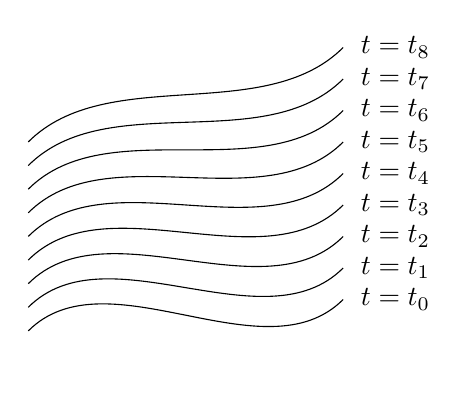
\begin{tikzpicture}
\foreach \s in {0,...,8}
{
\coordinate (A) at (0,0.3*\s);
\draw (A)  ..controls ++(1,1) and ++(-1,-1) .. ++(4,{0.4+0.1*\s}) node[right = 1mm] {$t=t_\s$}; %.. controls (1,4) and (3,0)
}
\end{tikzpicture}

  \caption{A foliation of spacetime in space-like slices along the time direction, with $t_i < t_j \forall i<j$.}
  \label{ch2:foliatefig}
\end{figure}  
  
  
  The organizing principle in usual QFT is labeling the representations with the eigenvalues of the casimir operators of the Poincar\'{e} algebra, $C_1=P_\mu P^\mu$ and $C_2=W_\mu W^\mu$, where $W_\mu$ is the Pauli-Lubanski operator. In a CFT however the operator $C_1$ is no longer a casimir, since it doesn't commute with, say, the generators of dilatations, $D$. If a representation contains a state with a fixed energy, due to scale invariance one can rescale the mass and energy by some constant factor and so the representation contains states of all energies. Therefore classification of states with respect to mass/energy is not feasible and moreover, in general for a CFT the hamiltonian, $P^0$ in general has a continuous spectrum. Instead, the dilatation operator $D$ plays the role of the Hamiltonian, and states in the Hilbert space live on surfaces of constant radius $r=r_0$ instead of constant time $t=t_0$. In direct analogy with the preceding discussion and eq. (\ref{ch2:transition_amplitude}) for general QFTs, the state $\ket{\{h_0(r=r_0)\}}$ living on the sphere $r=r_0$ evolves into the state $\ket{\{h_1(r=r_1)\}}$ given by:
  \begin{align} 
   \ket{\{h_1(r=r_1)\}} &= e^{-\beta D} \ket{\{h_0(r=r_0)\}} \label{ch2:radial_transition_amplitude_1} \\
			&= \mathbb{1} \, e^{-\beta D} \ket{\{h_0(r=r_0)\}} \\
			&= \int [\mathcal{D}h(r_1)] \ket{\{h(r_1)\}} \braket{\{ h(r_1)\}| e^{-\beta D} |\{h_0(r_0)\}} \\
			&= \int [\mathcal{D}h(r_1)] \ket{\{h(r_1)\}} \int_{\tilde{h}(r=r_0)=h_0(r_0)}^{\tilde{h}(r=r_1)=h(r_1)}[\mathcal{D}\tilde{h}] e^{-S[\tilde{h}]}  \\
			&= \left(\int_{h(r=r_0)=h_0(r_0)} [\mathcal{D}h(r_0 \leqslant r \leqslant r_1)] e^{-S[h]} \right) \ket{\{h(r_1)\}} \label{ch2:radial_transition_amplitude_2}
  \end{align}
  In particular one may ``create'' the vacuum state $\ket{0}$ using the path integral. Recall that in the limit that $\beta \to \infty$, the evolution operator (or transfer matrix, in statistical physics) $e^{-\beta \hat{D}}$ projects onto the ground state:
  \begin{align}
  e^{-\beta \hat{D}} \xrightarrow{\beta \to \infty} e^{-\beta E_0} \ket{0}\bra{0}
  \end{align}
  
  Since $r \to 0$ corresponds to taking the euclidean time $\tau \to -\infty \implies \beta \to \infty$, we have with eq.(\ref{ch2:radial_transition_amplitude_1} - \ref{ch2:radial_transition_amplitude_2}):
  \begin{align} 
   \ket{0} =\lim_{r_0\to \infty} \int [\mathcal{D}h_0(r_0)]\int [\mathcal{D}h(r_1)] \ket{\{h(r_1)\}} \int_{\tilde{h}(r=r_0)=h_0(r_0)}^{\tilde{h}(r=r_1)=h(r_1)}[\mathcal{D}\tilde{h}] e^{-S[\tilde{h}]} \label{ch2:radial_transition_amplitude_3}
  \end{align}
  
  This can be represented in the following form with the understanding that the boundary value configurations given by $h(r=r_1)$ are integrated over:
  
  \begin{align} \label{ch2:vac}
   \ket{0} = \int [\mathcal{D}h(r \leqslant r_1)] e^{-S[h]} \ket{\{h(r_1)\}}
  \end{align}

  
  With this expression in hand, we are set to discuss the \textbf{state-operator correspondence}.
  
  \subsubsection{State-Operator Correspondence}
  The State-Operator correspondence in CFT is a one-to-one correspondence between Hilbert space states living on the surface of some radius $r_0$ and operators inserted at the origin, or more generally anywhere in the region $r \leqslant r_0$. 
  
  
  
  \begin{enumerate}
   \item \textbf{Operator $\rightarrow$ State} Inserting an operator $\hat{\mathcal{O}}_{\Delta}(0)$ at the origin creates an eigenstate of the dilatation operator $\hat D$ on the sphere of radius $r_0$. In eq.(\ref{ch2:vac}) this corresponds simply to an insertion of the operator in the path integral:
   \begin{align}
   \hat{\mathcal{O}}_{\Delta}(0) \ket{0} = \left(\int [\mathcal{D}h(r \leqslant r_1)] \mathcal{O}_\Delta (0) e^{-S[h]} \right)\ket{\{h(r_1)\}}
   \end{align}
   \begin{align}
    \hat D \hat{\mathcal{O}}_{\Delta}(0) \ket{0} &= [\hat D , \hat{\mathcal{O}}_{\Delta}(0)] \ket{0} +  \cancelto{0}{\hat{\mathcal{O}}_{\Delta}(0) \hat D \ket{0}} \\
    &=\lim_{x\to 0} (\Delta -ix^\mu \partial_\mu) \hat{\mathcal{O}}_{\Delta}(x) \ket{0} \\
    &=\Delta \hat{\mathcal{O}}_{\Delta}(x) \ket{0}
   \end{align}
  
  Moreover, inserting an operator $\hat{\mathcal{O}}_{\Delta}(x)$ at a point $x$ inside the sphere of radius $r_0$, i.e. $0<|x|<r_0$ does not produce an eigenstate of the dilatation operator but since it is still a state in the Hilbert space it may be expanded in $\hat D$ eigenstates. This can be seen using the fact that $\hat P^\mu$ generates translations along $x^\mu$ and therefore $\hat{\mathcal{O}}_{\Delta}(x)= e^{i\hat{P}\cdot x}\hat{\mathcal{O}}_{\Delta}(0) e^{-i\hat{P}\cdot x}$ which gives:
  
  \begin{align}
   \hat{\mathcal{O}}_{\Delta}(x) \ket{0} &= e^{i\hat{P}\cdot x}\hat{\mathcal{O}}_{\Delta}(0) e^{-i\hat{P}\cdot x} \ket{0} \\
   &=e^{i\hat{P}\cdot x}\hat{\mathcal{O}}_{\Delta}(0) \ket{0} \\
   &=e^{i\hat{P}\cdot x} \ket{\Delta} \\
   &=\sum_{n=0}^\infty \frac{(i\hat{P}\cdot x)^n}{n!} \ket{\Delta} \\
   &= c_0(x) \ket{\Delta} + c_1(x) \ket{\Delta+1} +c_2(x) \ket{\Delta+2} \dots
  \end{align}
  Where in the second line we have used the uniqueness and conformal invariance of the vacuum $\ket{0}$ implying $\hat{P}^\mu \ket{0} = 0$. Therefore the only term surviving in  $e^{-i\hat{P}\cdot x} \ket{0}$ is the first term $\mathbb{1}\ket{0}$ with the identity operator. In the last line we have used the fact that $\hat{P}^\mu$ are raising operators for $\hat D$ eigenstates. This means $\hat P \ket{\Delta} \sim \ket{\Delta+1}, \hat{P}^2 \ket{\Delta} \sim \ket{\Delta+2}$ and so on.
  
  Another way to reach the same conclusion is using the path integral expression (\ref{ch2:vac}):
  \begin{align}
   \ket{\Psi}=\hat{\mathcal{O}}_{\Delta}(x) \ket{0} = \underbrace{\left(\int [\mathcal{D}h(r \leqslant r_1)] \mathcal{O}_\Delta (x) e^{-S[h]} \right)}_{\text{I}}\ket{\{h(r_1)\}}
   \end{align}
   
   The path integral (I) we can taylor expand $\mathcal{O}_\Delta (x)$ around $x=0$ to give:
  \begin{multline}
   \ket{\Psi} = \bigg( \int [\mathcal{D}h(r \leqslant r_1)] \bigg\lbrace \mathcal{O}_\Delta (0) + \frac{x}{1!}\partial \mathcal{O}_\Delta (0)  \\ 
   + \frac{x^2}{2!}\partial^2 \mathcal{O}_\Delta (0)+\dots \bigg\rbrace e^{-S[h]} \bigg)\ket{\{h(r_1)\}}
   \end{multline} 
   \begin{align}
    \implies \ket{\Psi} &= \sum_{n=0}^{\infty} \frac{(ix\hat P)^n}{n!}\bigg( \int [\mathcal{D}h(r \leqslant r_1)]  \mathcal{O}_\Delta (0) e^{-S[h]} \bigg)\ket{\{h(r_1)\}} \\
    \ket{\Psi} &= \sum_{n=0}^{\infty} \frac{(ix\hat P)^n}{n!} \hat{\mathcal{O}}_\Delta(0)\ket{0} \\
    \ket{\Psi} &= \sum_{n=0}^{\infty} \frac{(ix\hat P)^n}{n!} \ket{\Delta}
   \end{align}
  \item \textbf{State $\rightarrow$ Operator} Given a state $\ket{\psi}$ on a sphere of radius $r_0$ (in radial quantization), one can cut out a small sphere $S_\epsilon$ of radius $\epsilon$ at the origin with the boundary conditions on $S_\epsilon$ defined by $\ket{\psi}$ in the following sense: using the eqn. (\ref{ch2:radial_transition_amplitude_2}) one writes the state $\ket{\psi}$ as:
  
  \begin{align}
   \ket{\psi} = \left( \int_{h(\epsilon)=h_0(\epsilon)} [\mathcal{D}h(\epsilon \leqslant r \leqslant r_0)]   e^{-S[\tilde{h}]} \right) \ket{\{h(r_1)\}}
  \end{align}
  Where the initial state $\ket{\{h_0(\epsilon)\}}$ is determined uniquely given $\ket{\psi}$. Due to conformal invariance the absolute size of $r_0$ does not matter. Additionally in contrast to a QFT without conformal invariance one can take the limit $\epsilon \to 0$ and then the state $\ket{\{h_0(\epsilon)\}}$ defines uniquely an operator $\hat{\mathcal{O}}_{\ket{\psi}}(0)$ as:
  
  \begin{align}
   \lim_{\epsilon \to 0} \ket{\{h_0(\epsilon)\}} = \lim_{\epsilon \to 0}\hat{\mathcal{O}}_{\ket{\psi}}(\epsilon) \ket{0}
  \end{align}
  In particular, a given $\hat{D}$ eigenstate $\ket{\Delta}$ on some sphere $S_{r_0}$ corresponds uniquely to the operator insertion $\op{O}_\Delta(0)$ at the origin independent of the radius $r_0$.
   \end{enumerate}
  
  
%   
%   
%   
%   
%   States are classified according to their scaling dimension $\Delta$ under the dilatation operator $D$. Since $P^\mu$ and $K^\mu$ act as raising and lowering operators respectively, for each $\Delta$ we have a lowest ``energy'' state $\ket{\Delta}$ called the \emph{\textbf{primary}} which is annhilated by the lowering operator:
%   \begin{align}
%    K^\mu \ket{\Delta} = 0
%   \end{align}
%   Each such primary, along with all states obtained by succesive applications of the raising operator $P^\mu$, called the \emph{\textbf{descendant}} states furnishes a representation of the conformal algebra. 
%   
%   [check Tong -string theory+cardy les houches]
%   As we discussed before, one of the features of a Conformal field theory is that there is no inherent mass scale in the theory. Therfore, the hamiltonian ends up having a continuum of eigenstates and the usual quantisation on the line is not so useful since one cannot define asymptotic states in the usual way. We will see that just as in usual QFTs one utilises the time-translation invariance, to foliate spacetime into equal time slices and quantise the theory on these qual time slices, in a CFT it is more natural to use the scale invariance of the theory, and quantise it on circles of equal radii $r_0$. The nthe role played by the Hamiltonian (generator of time translations) is replaced by $D$ the generator of dilatations (scale transformations). Then $D$ has a discrete spectrum. So far we have discussed the canonical picture. 
%   
%   
%   
% 
%   
%   In the path integral formulation, the Hilbert space of such a CFT would correspond to the space of field configurations $\Ket{h(r_0,\theta)}$ on a circle of radius $r_0$ \cite{Cardy:2008jc}. [CLARIFY]. The vacuum state is given by
%   
%   
%   Let us discuss the Hilbert Space structure of QFTs. In canonical quantisation of a QFT, the usual procedure is to choose a foliation of space-time into spacelike slices of constant time. Each leaf of this foliation carries its own copy of Hilbert space.[insert diagram]. Since the Hilbert spaces on different slices are related by a symmetry transformation, namely that of time translation, generated by $P^0$, the Hilbert spaces are infact isomorphic and can be identified as the same Hilbert space. The Hamiltonian ($P^0$) and $P^i$ form a complete set of commuting operators (CSCO) in the Poincar\'{e} algebra, therefore we can classify states according to their eigenvalues i.e. the energy and momenta:
%   
%   \begin{align}
%    P^\mu \Ket{k^\mu} = k^\mu \Ket{k^\mu}
%   \end{align}
%   
%   
%   
%   
%   
%   Then there exists a vacuum state $\left| \text{VAC} \right\rangle$ which is annhilated by the lowering operator, and \emph{fields} or \emph{field operators} map one state in the Hilbert space into another state. For two states, $\left| \psi_1 \right\rangle$ and $\left| \psi_2 \right\rangle$ on the same slice, the probability of one state evolving into another is given by the overlap of these $\left\langle \psi_2 | \psi_1 \right\rangle$, and this also measures the correlator of the two operators which generate these states. So if $\left| \psi_1 \right\rangle = \mathcal{O}_1 \left| \text{VAC} \right\rangle$ and $\left| \psi_2 \right\rangle = \mathcal{O}_2 \left| \text{VAC} \right\rangle$, then we have:
%   \begin{align*}
%    \left\langle \psi_2 | \psi_1 \right\rangle = \left\langle \mathcal{O}_2 \mathcal{O}_1 \right\rangle
%   \end{align*}
% 
%   
%   One may insert field operators on a particular time slice, and this may correspond to generating or measuring a particle. For example, one may insert a creation operator $a^{\dag}_p$ on the vacuum of the $t=-T$ slice to get the $\left| \text{in} \right\rangle$ state: 
%   \begin{align*}
%    \left| \text{in} \right\rangle= \left|\vec{p},-T \right\rangle = a^{\dag}_{\vec{p}} \left| \text{VAC}, -T \right\rangle
%   \end{align*}
% and similarly the out state on the  $t=+T$ 
% \begin{align*}
%  \left\langle \text{out} \right| = \left\langle \vec{q},T \right| = \left\langle \text{VAC}, T \right| a_{\vec{q}}
% \end{align*}
%   The time evolution operator $U(t_2,t_1)$ can propagate states from time slice $t_1$ to another time slice $t_2$ and thus we can calculate the probability amplitude of  project one state $\psi_1$ on another state $\psi_2$ and get the probability amplitude for this 
%   
%   One typically wants to study 2 dimensional CFTs on the cylinder since this is the natural home of a CFT for example in String Theory and moreover it removes IR divergences. This essentially amounts to compactifying the space direction using periodic boundary conditions (insert diagram). Now this 
%   
   
  \subsection{Operator Product Expansion}
  
  Let's go ahead and see a general derivation of the operator product expansion in CFTs from radial quantization. The crucial difference of the CFT OPE from general QFT OPE is the following: for a general QFT the OPE is an asymptotic expansion of the product of two operators $\phi_1(x_1), \phi_2(x_2)$ inside the correlator, in the limit when the two operators get arbitrarily close, $x_1 \to x_2$. However, in a CFT, the OPE is convergent and is an exact statement. Inside a correlator, the radius of convergence of the OPE is given by the next nearest operator insertion.
  
  \begin{figure}
\centering
\begin{tikzpicture}
\draw[dashed] (0,0) circle (3cm);
\coordinate (A) at (45:3);
\draw[fill] (0,0) node[below]{$\mathcal{O}_1(x_1)$} circle (0.05cm);
\draw[fill] (1.5,0.5) node[below]{$\mathcal{O}_2(x_2)$} circle (0.05cm);
\draw[fill] (A) node[right]{$\mathcal{O}_3(x_3)$} circle (0.05cm);
\draw[fill] (4,-1) node[below]{$\mathcal{O}_4(x_4)$} circle (0.05cm);
\end{tikzpicture}
\caption{The radius of convergence of the $\mathcal{O}_1\mathcal{O}_2$ OPE is determined by the next nearest operator insertion. In this case it is given by $r=|x_1-x_3|$.}
\end{figure}
  
  Using the path integral expressions of the State-Operator correspondence we can write for the state $\ket{\Psi}$(see fig. \ref{ch2:pic:OPEderive}):
  
  \begin{align}
   \ket{\Psi} = \hat{\mathcal{O}}_2(x) \hat{\mathcal{O}}_1(0) \ket{0} =\int [\mathcal{D}h(r\leqslant r_0)] \mathcal{O}_2(x) \mathcal{O}_1(0) e^{-S[h]} \ket{\{h(r_1)\}}
  \end{align}

  \begin{figure}
\label{ch2:pic:OPEderive}
\centering
\begin{tikzpicture}
\draw[dashed] (0,0) circle (3cm);
\coordinate (A) at (45:3);
\draw[fill] (0,0) node[below]{$\mathcal{O}_1(0)$} circle (0.05cm);
\draw[fill] (-1.7,0.8) node[below]{$\mathcal{O}_2(x)$} circle (0.05cm);
%\draw[fill] (A) node[right]{$\mathcal{O}_3(x_3)$} circle (0.05cm);
%\draw[fill] (4,-1) node[below]{$\mathcal{O}_4(x_4)$} circle (0.05cm);
\draw[fill] (A) node[right] {$\ket{\Psi}$};
\end{tikzpicture}
\caption{Derivation of the OPE using the State-Operator correspondence.}
\end{figure}
  
  This state $\ket{\Psi}$ being an element of the Hilbert space (and a function of the coordinate $x$) may be expanded in eigenvectors (primaries and descendants) of the operator $\hat D$, $D_n$
  
  \begin{align}
   \ket{\Psi} = \sum_{n} c_n(x) \ket{D_n}
  \end{align}

  Using the state-operator correspondence now we can associate each $\ket{D_n}$ either a \textbf{primary operator}  $\hat{\mathcal{O}}$ or some descendant $\partial^n \hat{\mathcal{O}}$:
  
  \begin{align} 
   \hat{\mathcal{O}}_2(x) \hat{\mathcal{O}}_1(0) \ket{0} &= \left(\sum_{{\mathcal{O}}} \sum_{n} c^{\mathcal{O}}_n(x,\partial^n) \hat{\mathcal{O}}(0) \right) \ket{0} \label{ch2:OPE_proof_1} \\
   &=\left(\sum_{{\mathcal{O}}}  \frac{\lambda_{21\mathcal{O}}}{|x|^k} [1+\frac{c_1}{2} x^\mu \partial_\mu +\frac{c_2}{8} x^\mu x^\nu \partial_\mu \partial_\nu + \dots]\op{O}_{\Delta}(0) \right) \ket{0} \label{ch2:OPE_proof_2}
  \end{align}
  Where the summation is over primaries $\op{O}$ and $[\dots]$ represent further descendants of the respective primaries which come with their own additional coefficients.

  Conformal symmetry makes the OPE even more powerful in that by requiring that both the LHS and RHS of eqn. (\ref{ch2:OPE_proof_1}) transform in the same way one can constrain the coefficients of particular operators in the OPE. In particular, by operating on both sides of \ref{ch2:OPE_proof_2} with $\hat D$ and matching the coefficients, one can fix the exponent $k$ for a scalar operator $\op{O}$ of dimension $\Delta$ in the OPE \ref{ch2:OPE_proof_2} to be $k=\Delta_1+\Delta_2-\Delta$, and by operating with $K^\mu$ recursively one can fix the constants $c_i$ exactly.
  \begin{multline}\label{ch2:OPE_final}
  \braket{\op{O}_1(x)\op{O}_2(0)}=\left(\sum_{{\mathcal{O}}}  \frac{\lambda_{21\mathcal{O}}}{|x|^{\Delta_1+\Delta_2 - \Delta}} [1+\frac{c_1}{2} x^\mu \partial_\mu +\frac{c_2}{8} x^\mu x^\nu \partial_\mu \partial_\nu + \dots]\op{O}_{\Delta}(0) \right) \ket{0} 
  \end{multline}

  
  \subsection{Embedding (Projective light cone) Formalism} \label{ch2:embedding}
  We saw in the last section that the D dimensional (global) euclidean conformal algebra turns out to be isomorphic to the D+2 dimensional Minkowski algebra SO(D+1,1). This inspires the so called Embedding Formalism for CFT. The idea here is to consider the D-dimensional euclidean space (on which the CFT lives) as a subspace of D+2 dimensional Minkowski space. Naturally, to successfully achieve this the most important requirement is that Lorentz transformations on the embedding space correspond to conformal transformations on the CFT subspace. We start with the following metric in Minkowski space. 
  \begin{align}
   ds^2 = -dY_{-1}^2 +dY_0^2 + \sum_{i=1}^D dY_i^2
  \end{align}
  
  As we will see, this considerably simplifies calculations since now the generators of the conformal algebra can be identified with the (linear) generators of minkowski algebra in D+2 dimensions.
  For this section, capital latin indices $M,N \in \{-1,0,1,\cdots D \}$ and represent variables in the embedding Minkowski space. Lower case greek indices $\mu,\nu \in \{1,2,\cdots D\}$ and represent variables in the D-dimensional euclidean CFT space. 
  
  Define the light cone coordinates as 
  
  \begin{align}
   Y_\pm &= Y_{-1} \pm Y_{0}
  \end{align}
  In lightcone coordinates the Minkowski metric becomes
  \begin{align}
   ds^2 = - dY_+ \cdot dY_- + \sum_{i=1}^D dY_i^2 
  \end{align}

   Now we have D+2 independent variables $Y^M$ and so we need 2 constraint equations to specify the subspace of the CFT. The first constraint comes from restricting to the light cone:
   
   \begin{align}
    Y^2=Y\cdot Y = Y^M Y_M = 0
   \end{align}
  This subspace is closed under Lorentz transformations which is a necessary condition to have, once we identify the D-dimensional conformal generators with the D+2 dimensional Lorentz generators.
  Define 
  \begin{align}
   Y^i = y^i \; : I \in \{1,2,\dots D \}
  \end{align}
  Then the lightcone condition implies
  \begin{align}
   Y_+ Y_- = |y|^2
  \end{align}

  The second constraint is imposed with the constraint of living on a \emph{Poincar\'{e} section} of the lightcone, given by $Y_+ = a$ where $a$ is some non-zero constant. Then the metric on this section is given by:
  \begin{align}
   ds^2 |_{Y_- = |y|^2/Y_+ , Y_+=a} = \sum_{i=1}^D dY_i^2 = \sum_{i=1}^D dy_i^2
  \end{align}
  
  And a general point on the section is given by:
  
  \begin{align}
   (Y_+,Y_-,Y^i) = \left( a,\frac{|y|^2}{a}, y^i \right)
  \end{align}

  
  Now the CFT lives on the null projective cone of this space, i.e. the surface given by non-zero, null vectors with rays identified
  \begin{align}
   Y^2=Y\cdot Y = Y^\mu Y_\mu &= 0 \\
   Y &\neq 0 \\
   Y \equiv aY ; a \in \mathcal{R}
  \end{align}


  \subsection{CFT Correlators}
  The basic data for any conformal field theory are the spectrum of (quasi) primary operators and their OPE coefficients. The basic structures of interest, referred to henceforth as 'observables', are the correlators. The primary fields in $d=2$ CFTs correspond to quasi-primary fields in $d > 2$ CFTs. 2 point correlators in CFTs are completely determined in the sense that upto a normalization constant, no dynamical input is necessary to calculate these correlators. The conformal group constrains the CFT correlators of (quasi) primary operators $\mathcal{O}_1$ and $\mathcal{O}_2$ such that the two point correlators are exactly determined, upto renormalization. 
  
  Due to translation and rotational invariance, $\braket{\op{O}_1(x)\op{O}_2(0)} = f(x)$ can only depend on the quantity $|x|^2$. Imposing scale covariance requires that the function $f$ transform homogeneously for some $\lambda \in \amsmathbb{R}^+$, i.e. $f(\lambda x)=\lambda^{-\Delta} f(x)$ for some appropriate $\Delta$. This fixes the correlator as:
  \begin{align}
   f(x) = \braket{\op{O}_1(x)\op{O}_2(0)} = \frac{c_{12}}{|x|^{2\Delta}}
  \end{align}
  Where special conformal transformations impose the condition $\text{dim}(\op{O}_1)=\text{dim}(\op{O}_2)=\Delta$, and so two quasi-primary fields can be correlated only when they have the same scaling dimensions. Normalizing the $\hat D$ eigenstates $\ket{\Delta}$ as $\braket{\Delta_1|\Delta_2}=\delta_{12}$ fixes $c_{12}=\delta_{12}$.
   \begin{align} \label{ch2:two_point}
   f(x) = \braket{\op{O}_1(x)\op{O}_2(0)} = \frac{\delta_{12}}{|x|^{2\Delta}}
  \end{align}
%   There are many ways to derive this, the one illustrated here however employs the OPE. Use the OPE on the operators $\op{O}_1\op{O}_2$ inside the correlator $\braket{0|\cdot|0}$ and then the only non-zero contribution comes from operators having $\ket{0}$ as an eigenstate, if the OPE has such an operator. 
%   $$
%   \braket{0| \op{O}_1(x) \op{O}_2(y)|0} = \frac{c_{12}}{|x-y|^{2\Delta}}
%   $$
  Similarly requiring that the 3-point function $\braket{\op{O}_1(x_1) \op{O}_2(x_2) \op{O}_3(x_3)}$ be invariant under translations and rotations and covariant under scale and special conformal transformations fixes their form as: 
  \begin{align} \label{ch2:3_point}
   \braket{ \op{O}_1(x_1) \op{O}_2(x_2) \op{O}_3(x_3)} = \frac{C_{123}}{|x_{12}|^{\Delta_1+\Delta_2-\Delta_3}|x_{23}|^{\Delta_2+\Delta_3-\Delta_1}|x_{31}|^{\Delta_3+\Delta_1-\Delta_2}}
  \end{align}
  Where the constants $C_{123}$ are exactly the the OPE coefficients $\lambda_{12\op{O}}$ for $\op{O}=\op{O}_3$.
%   
%   \begin{multline}
%   \braket{ \op{O}_1(x_1) \op{O}_2(x_2) \op{O}_3(x_3)} = \sum_{{\mathcal{O}}}  \frac{\lambda_{21\mathcal{O}}}{|x_{12}|^{\Delta_1+\Delta_2 - \Delta}} \bigg(\braket{\op{O}_{\Delta}(x_2) \op{O}_{3}(x_3)}+ \dots \bigg)   \\  \frac{c_{123}}{|x_{12}|^{2\Delta}}
%   \end{multline}
%   Using the OPE (\ref{ch2:OPE_final}) and the 2 point function (\ref{ch2:two_point}) we can derive the 3-point function:
  
  This means that for 2 and 3 point correlators in CFT, the spacetime dependence is uniquely determined by conformal symmetry with no dynamical information of the theory. In fact the only free parameters (not fixed by conformal symmetry) in the OPE (\ref{ch2:OPE_final}) are the OPE coefficients $\lambda_{ijk}$.
  

  %\subsection{Modular Invariance and Crossing Symmetry}
  \section{Part II: Conformal Blocks}
  
    For 4-point correlators, things get even more interesting. One may construct functions of the coordinates of operator insertions, $x_i$, called conformal invariants. These conformal invariants as the name suggests are invariant under conformal transformations. In $d$ dimensions there exist 2 distinct conformal invariants for 4 points $u,v$ given by:
  
  \begin{align} \label{ch2:cross_ratios}
   u=\frac{|x_{12}|^2 |x_{34}|^2}{|x_{13}|^2|x_{24}|^2},\quad v=\frac{|x_{14}|^2|x_{23}|^2}{|x_{13}|^2|x_{24}|^2}
  \end{align}

  
  4-point correlators contain dynamical information about the CFT, however there are functions called conformal blocks which contain all the information fixed by conformal symmetry in a 4-point correlator. This can be understood as an expansion of the 4-point correlator with the conformal blocks as expansion functions (also called basis functions).
  
  The most straightforward way to look at this is using the OPE. To calculate the four point function $\braket{ \op{O}_1(x_1) \op{O}_2(x_2) \op{O}_3(x_3) \op{O}_4(x_4)}$, as illustrated in figure (\ref{ch2:blocks_fig}) one can expand in the $\op{O}_1 \op{O}_2$ and $\op{O}_3 \op{O}_4$ OPEs after which one is left with two point functions of the exchanged operators.
  \begin{figure}[!h] \label{ch2:blocks_fig}
\centering
\begin{tikzpicture}[scale=2,>=stealth]
%Draw Circle radius 1 cm
  \def\radi{1cm}
    \coordinate (O1) at (0,0);
    \coordinate (O2) at (1,0);
   % \foreach \angle/\count in {45/1,135/2,225/3,315/4}
    %    {
        
\tikzset{snake it/.style={decorate, decoration=snake}}
%Draws the 3 acceleration vectors directed inward and offset slightly from the distance vectors
       % \draw [name=acceleration vectors,very thick, snake it]
        %    (\angle:1.2cm) -- node[midway] {} (\angle:0.9cm) ;
         %     \path [draw=blue,snake it](-4,0) -- (-2,0) -- (2,0) -- (4,0);
  %\draw[draw=blue, snake it] (2,0) arc (0:180:2cm);
   % } snake it
    
        \path[coordinate] (O2)  coordinate(A)++( 45:\radi) coordinate(B1);
        \path[coordinate] (O1)  coordinate(A)++( 135:\radi) coordinate(B2);
        \path[coordinate] (O2)  coordinate(A)++( -45:\radi) coordinate(B3);
        \path[coordinate] (O1)  coordinate(A)++( -135:\radi) coordinate(B4);
        \draw[draw=red, very thick] (O2)--(B1);
        \draw[draw=red, very thick] (O2)--(B3);
        \draw[draw=red, very thick] (O1)--(B2);
        \draw[draw=red, very thick] (O1)--(B4);
        \draw[draw=red,very thick] (O1)--(O2);
        
         \draw (0.5,0) node[above]{$\Delta$};
         \draw (B2) node[above]{$i$};
         \draw (B4) node[below]{$j$};
         \draw (B3) node[below]{$k$};
         \draw (B1) node[above]{$l$};
         
         \draw (-2.5,0) node[center]{\Large $\braket{\op{O}_i\op{O}_j\op{O}_k\op{O}_l}=\displaystyle\sum_{\Delta} \lambda_{ij\Delta} \lambda^{kl\Delta}$  };
\end{tikzpicture}
\caption{4-point correlator as a sum over conformal partial waves, weighted by the OPE coefficients.}
\end{figure}
  
  \begin{multline}
   \braket{ \op{O}_1(x_1) \op{O}_2(x_2) \op{O}_3(x_3) \op{O}_4(x_4)} = \\ \sum_{\op{O}} \sum_{\op{O}^\prime} \frac{\lambda_{12\op{O}}}{|x_{12}|^{\Delta_1+\Delta_2-\Delta}} \frac{\lambda_{34\op{O}^\prime}}{|x_{34}|^{\Delta_3+\Delta_4-\Delta^\prime}} \Braket{\bigg( \op{O}(x_2)+\dots \bigg) \bigg( \op{O}^\prime(x_4)+\dots\bigg)}
  \end{multline}
  
  \begin{align}
  &= \sum_{\op{O}}  \frac{\lambda_{12\op{O}}}{|x_{12}|^{\Delta_1+\Delta_2-\Delta}} \frac{\lambda_{34\op{O}}}{|x_{34}|^{\Delta_3+\Delta_4-\Delta}} \bigg( \braket{\op{O}(x_2)\op{O}(x_4)}+\braket{\partial \op{O}(x_2) \partial \op{O}(x_4)}+\dots \bigg) \label{ch2:CPW_0}\\
  &= \sum_{\op{O}}  \frac{\lambda_{12\op{O}}}{|x_{12}|^{\Delta_1+\Delta_2-\Delta}} \frac{\lambda_{34\op{O}}}{|x_{34}|^{\Delta_3+\Delta_4-\Delta}} \bigg( \frac{1}{|x_{24}|^{2\Delta}}+\dots \bigg) \label{ch2:CPW_1}\\
   &=\sum_{\Delta}  \lambda_{12\Delta} \lambda_{34\Delta} W_{\Delta,l}(x_i) \label{ch2:CPW_2}
  \end{align}
  These $W_{\Delta,l}(x_i)$ are called Conformal Partial Waves (CPW) and are uniquely fixed by conformal covariance. Each CPW receives contributions from the entire conformal family of the primary with scaling dimension $\Delta$ and spin $l$. The contributions of the descendant 2-point functions are denoted by $\dots$ in eqn. (\ref{ch2:CPW_1}). These CPWs are closely related to Conformal Blocks, in that where CPWs are conformally \emph{covariant} and depend on the relative distance $|x_{ij}|$, conformal blocks are conformally \emph{invariant} and are functions of the conformal invariant cross ratios $u,v$ (\ref{ch2:cross_ratios}). These two differ only by a scale factor. Denoting conformal blocks by $G_{\Delta,l}(u,v)$, the relationship between the two is given by:
  \begin{align} \label{ch2:CPW}
   W_{\Delta,l}(x_i)=\frac{1}{{x_{12}^2}^{\frac{1}{2}(\Delta_1+\Delta_2)}{x_{34}^2}^{\frac{1}{2}(\Delta_3+\Delta_4)}} \left(\frac{x_{14}^2} {x_{13}^2}\right)^\frac{\Delta_{34}}{2} \left(\frac{x_{24}^2}{x_{14}^2}\right)^\frac{\Delta_{12}}{2} G_{\Delta,l}(u,v)
  \end{align}
  
  For two dimensional CFTs one can make a stronger statement, which is that the CPWs (and conformal blocks) factorize into holomorphic and anti-holomorphic parts. It is usual to simplify the expressions by using conformal invariance to send $z_1 \to \infty, z_2 \to 1 \text{ and}, z_3 \to 0$ such that the functional dependence on coordinates is simplified:
  \begin{align}
   \braket{\op{O}_1(\infty,\infty)\op{O}_2(1,1)\op{O}_3(z,\bar{z})\op{O}_4(0,0)}= \sum_{\Delta}  \lambda_{12\Delta} \lambda_{34\Delta} \mathcal{F}(h_i,\Delta;z) \bar{\mathcal{F}}(\bar{h}_i,\bar{\Delta};\bar{z})
  \end{align}

% 
%    four point fucntions, on the other hand \cite{Hijano:2015rla} \cite{Hijano:2015zsa} 
%   
%   The four point function of four scalar primaries $\phi_i$ with scaling dimensions $\Delta_i$ is given by:
%   \begin{align}
%    \left\langle \phi_1(x_1) \phi_2(x_2) \phi_3(x_3) \phi_4(x_4)\right\rangle = \frac{1}{{x_{12}^2}^{\frac{1}{2}(\Delta_1+\Delta_2)}{x_{34}^2}^{\frac{1}{2}(\Delta_3+\Delta_4)}} \left(\frac{x_{14}^2} {x_{13}^2}\right)^\frac{\Delta_{34}}{2} \left(\frac{x_{24}^2}{x_{14}^2}\right)^\frac{\Delta_{12}}{2} F(u,v) \tag{4p}
%   \end{align}
%   The function $F$ can be expanded as a sum over conformal blocks $G_{\Delta,l}(u,v)$:
%   \begin{align*}
%    F(u,v)=\sum_{\mathcal{O}} C_{12\mathcal{O}}C_{34}^{\mathcal{O}} G_{\Delta,l}(u,v)
%   \end{align*}
%   Where $\mathcal{O}$ is a primary with scaling dimension $\Delta$ and spin $l$. Here the conformal block recieves contributions from the primary $\mathcal{O}$ and all it's descendants.
%   Where $u,v$ are the two independent conformally invariant cross ratios:
%   \begin{align*}
%    u = \frac{x_{12}^2 x_{34}^2}{x_{13}^2x_{24}^2}, v= \frac{x_{14}^2x_{23}^2}{x_{13}^2 x_{24}^2}
%   \end{align*}

  %\subsection{Recursion Relations}
  \subsection{Integral Representations}
  Illuminating integral representations for conformal blocks were obtained by Ferrara, Gatto, Grillo and Parisi in \cite{Ferrara:1,Ferrara:2,Ferrara:3}. We just state the results and refer the reader to the original literature for a more detailed discussion. For the exchange of a spinless operator ($l=0$) with scaling dimension $\Delta$, and also spinless external operators $\op{O}_i$, the conformal block $G_{\Delta,0}$ can be written in an integral form as:
  \begin{multline}
   G_{\Delta,0}=\frac{1}{2\beta_{\Delta 34}} u^{\Delta/2} \int_0^1 d \sigma \sigma^{\frac{\Delta + \Delta_{34}-2}{2}} (1-\sigma)^{\frac{\Delta - \Delta_{34}-2}{2}} (1-(1-v)\sigma)^{\frac{-\Delta + \Delta_{12}}{2}} \\ \times \tensor[_2]{F}{_1}\left(\frac{\Delta+\Delta_{12}}{2},\frac{\Delta-\Delta_{12}}{2},\Delta-\frac{d-2}{2},\frac{u\sigma(1-\sigma)}{1-(1-v)\sigma} \right)
  \end{multline}
  with
  \begin{align}
   \beta_{\Delta 34} \equiv \frac{\Gamma\left(\frac{\Delta+\Delta_{34}}{2} \right) \Gamma\left( \frac{\Delta-\Delta_{34}}{2}\right)}{2\Gamma(\Delta)}
  \end{align}


%   \chapter{Introduction to 2+1 Gravity}
%   \section{Review}
%   \section{BTZ black holes and Conical Defects}
%   \section{Chern-Simons formulation}
%   \cite{Achucarro:1987vz}

\chapter{Conformal Blocks using CFT}

Despite being well defined functions as sum over two point functions of conformal families, practical computation of Conformal Blocks is far from trivial. Over the years, various techniques have been developed to calculate explicit expressions for conformal blocks where possible; series expansions and recursive formulas where not. This chapter lists two powerful CFT methods for calculation of conformal blocks in various limits. 

The Conformal Casimir approach gives a differential equation that must be satisfied by any conformal block, and has been used to calculate explicit expressions for conformal blocks (in terms of hypergeometric functions) for $d=even$ conformal field theories. We will use this in Chapter \ref{ch:holographic} to verify that the holographic expression obtained indeed calculates the conformal block with the claimed exchanged conformal family.

The monodromy method calculates the semi-classical (central charge $c \to \infty$) conformal block by imposing a required monodromy on the solutions of a particular differential equation. Concisely, we solve the differential equation and then impose the required monodromy to determine a certain \emph{auxiliary function} $c_2(x_i)$ whose indefinite integral directly computes the 4-point conformal block. 

In general the difficulty goes up as one goes to more complicated representations of the conformal group. It is much harder to calculate conformal blocks due to an exchange of a spinning operator with the external operators carrying spin as well, as compared to calculating conformal blocks for the case where all operators are spinless. Moreover CFT$_d$ conformal blocks for even $d$ and scalar exchange can be resummed into hypergeometric functions \cite{Hijano:2015zsa}. No such representation is known for odd $d$.

\section{Conformal Casimir Approach}
The idea in the Conformal Casimir approach is that the conformal partial waves $W_{\Delta,l}(x_i)$ \ref{ch2:CPW} are solutions of a second order differential equation formed from the Conformal Casimir. This can be taken as a definition of the CPWs and can be used to explicitly calculate conformal blocks, where possible.

This section is formulated in the Embedding formalism (section \ref{ch2:embedding}) since the relevant equations appear in a simpler form in this formalism. In the Embedding formalism, one identifies $d$-dimensional conformal group generators with $d+2$-dimensional Lorentz group generators $L_{AB}$. Then the operator $L^2=L_{AB}L^{AB}$ is the casimir of the algebra. This means that all descendant states $(\hat{P}^\mu)^n\ket{\Delta}$ belonging to the conformal family of the primary $\ket{\Delta} = \op{O}\ket{0}$ have the same eigenvalue given by \cite{Dolan:2000ut}: 

\begin{align}
 C_2(\Delta,l)= - \Delta(\Delta-d)-l(l+d-2)
\end{align}

As for usual conformal group generators, the action of $L_{AB}$ on operators $\op{O}_1(x_1)$ is the application of a differential operator on the operator $\op{O}_1(x_1)$:

\begin{align} \label{ch3:casimir_action}
 [L_{AB},\op{O}_1(x_1)] = L^1_{AB}\op{O}_1(x_1)
\end{align}

Where $L_{AB}^1$ represents the differential operator w.r.t the position $x_1$. Using \ref{ch3:casimir_action} and the invariance of the vacuum under conformal transformations $L_{AB}\ket{0}=0$ one can write for the conformal casimir $L^2$ and some general state $\ket{\alpha}$:

\begin{align} \label{ch3:differential_casimir}
 \braket{0|\op{O}_1(x_1)\op{O}_2(x_2)L^2|\alpha} = (L_{AB}^1+L_{AB}^2)^2\braket{0|\op{O}_1(x_1)\op{O}_2(x_2)|\alpha}
\end{align}

with the differential operator on the RHS defined as 

\begin{align}
 (L_{AB}^1+L_{AB}^2)^2 \equiv \frac{1}{2}(L_{AB}^1+L_{AB}^2)(\tensor[]{L}{^1^{AB}}+\tensor[]{L}{^2^{AB}})
\end{align}

Consider expression \ref{ch2:CPW_0} for a 4-point function, reproduced here for clarity:

\begin{multline}
 \braket{ \op{O}_1(x_1) \op{O}_2(x_2) \op{O}_3(x_3) \op{O}_4(x_4)} \\ =  \sum_{\op{O}}  \frac{\lambda_{12\op{O}}}{|x_{12}|^{\Delta_1+\Delta_2-\Delta}} \frac{\lambda_{34\op{O}}}{|x_{34}|^{\Delta_3+\Delta_4-\Delta}} \bigg( \braket{\op{O}(x_2)\op{O}(x_4)}+\braket{\partial \op{O}(x_2) \partial \op{O}(x_4)}+\dots \bigg)
\end{multline}

This is equivalent to inserting the identity corresponding to the complete set of projection operators:

\begin{align}
 \mathbb{1} = \sum_{\op{O} \text{ primary}} \sum_{n=0}^\infty \ket{P^n \op{O}}\bra{P^n \op{O}}
\end{align}
\begin{multline}
 \braket{ \op{O}_1(x_1) \op{O}_2(x_2) \mathbb{1}  \op{O}_3(x_3) \op{O}_4(x_4)} = \sum_{\op{O} \text{ primary}} \sum_{n=0}^\infty \braket{0| \op{O}_1(x_1) \op{O}_2(x_2)|P^n \op{O}}  \braket{P^n \op{O}| \op{O}_3(x_3) \op{O}_4(x_4)|0}
\end{multline}

Comparing to eqn. \ref{ch2:CPW_2} we get for the CPW due to exchange of operator $\op{O}$ with scaling dimension and spin $\Delta, l$ respectively:

\begin{align}
 W_{\Delta,l}(x_i) = \frac{1}{\lambda_{12\Delta} \lambda_{34\Delta}} \sum_{n=0}^\infty \braket{0| \op{O}_1(x_1) \op{O}_2(x_2)|P^n \op{O}}  \braket{P^n \op{O}| \op{O}_3(x_3) \op{O}_4(x_4)|0}
\end{align}

With eqn. \ref{ch3:differential_casimir} and the fact that $L^2 \ket{P^n \op{O}} = C_2(\Delta,l)\ket{P^n \op{O}} \, \forall \, n \in \amsmathbb Z_{\ge 0}$ we have
\begin{align}
 (L_{AB}^1+L_{AB}^2)^2 W_{\Delta,l}(x_i) = \frac{C_2(\Delta,l)}{\lambda_{12\Delta} \lambda_{34\Delta}} \sum_{n=0}^\infty \braket{0| \op{O}_1(x_1) \op{O}_2(x_2)|P^n \op{O}}  \braket{P^n \op{O}| \op{O}_3(x_3) \op{O}_4(x_4)|0}
\end{align}

\begin{align}
 \implies (L_{AB}^1+L_{AB}^2)^2 W_{\Delta,l}(x_i) = C_2(\Delta,l) W_{\Delta,l}(x_i) 
\end{align}

The Lorentz killing vectors $L_{AB}$ are written as  $L_{AB}= Y_A \partial_B-Y_B \partial_A$ which implies that for $Y$ on the AdS hyperbola $Y^2=-1$ ,

\begin{align}
 L^2 f(Y) = \frac{1}{2}L_{AB}L^{AB} f(Y) = - \nabla_Y f(Y)
\end{align}

This will serve as a useful CFT check for the Witten diagram calculation of conformal blocks in the next chapter.

\section{Monodromy Method}



The monodromy method is a technique to calculate conformal partial waves for 2-D CFTs in the semi-classical limit. The semi-classical limit for 2D CFTs corresponds to taking the central charge $c \to \infty$. This is the main limit of interest in this thesis, and the motivation for this limit and the holographic calculation of conformal blocks in this limit is included in chapter \ref{ch:semiclassical}. The monodromy method and the terms 'semi-classical limit', 'heavy' and 'light' operators come from Liouville theory which is a CFT with a specific action (see \cite{Harlow:2011ny} for a detailed discussion of Liouville theory and \cite{Harlow:2011ny,Fitzpatrick:2014vua,Hartman:2013mia} for the Monodromy method). However the idea is that since the conformal blocks are determined solely by the Virasoro algebra, they apply for any CFT at large central charge\cite{Hartman:2013mia}.

The word monodromy come from greek \emph{mono} meaning 'alone' or 'singly' and \emph{dr\'omos} meaning 'to run'. The monodromy group of a complex differential equation specifies the behaviour of the solutions after going around a singularity once. More precisely, given the following linear differential equation 
  \begin{align} \label{ch3:linear_system}
   \frac{d\bold{y}}{dz}=A\bold{y}
  \end{align}
 with $A \in GL_n(\amsmathbb{C}[z])$ and $\bold{y}$ a $n$-vector, let $S=\{a_0,a_1,\dots,a_s\}$ be the set of singular points of $A$. Let $b_0 \in \amsmathbb{P}^1(\amsmathbb{C})\setminus S$ where  $\amsmathbb{P}^1(\amsmathbb{C})$ is the complex Riemann sphere. Then standard existence and uniqueness theorems imply a $n\times n$ solution matrix $Y$ (the columns of $Y$ are the solutions $\bold{y}_1,\bold{y}_2,\dots,\bold{y}_n$) in the neighbourhood of $b_0$. Choose a closed path $\gamma$ starting and ending at $b_0$ and encircling one of the singularities, say $a_0$. Analytically continue the solution matrix $Y$ to $\tilde{Y}$ along the path $\gamma$ back to the point $b_0$. Then $\tilde{Y}$ and $Y$ are related by a constant matrix $M$ called the \emph{monodromy matrix}:
 
 \begin{align}
  \tilde{Y} = M Y
 \end{align}
 
It is expected that in the semi-classical $c \to \infty$ limit the conformal partial waves exponentiate, although as of yet there exists no direct proof from the definition of conformal partial waves as sum over conformal family contributions. 
\begin{align} \label{ch3:semiclassical_exponentiation}
 \braket{0|\op{O}_1(x_1)\op{O}_2(x_2)|\alpha}\braket{\alpha|\op{O}_3(x_3)\op{O}_4(x_4)|0} = \mathcal{F}_{\alpha}(x_i) \approx e^{-\frac{c}{6}f(x_i)}
\end{align}

The main result of this section is that to determine the function $f(x_i)$ in \ref{ch3:semiclassical_exponentiation}, we need to solve the following differential equation

\begin{align} \label{ch3:monodromy_diff}
 \psi^{\prime\prime}(z)+T(z)\psi(z)=0
\end{align}
with $T(z)$ not completely known, but dependent on a particular function $c_2(x_i)$ (to be determined). Then impose a specific monodromy determined by the conformal weights of the operators $\op{O}_i$ in \ref{ch3:semiclassical_exponentiation} on the two solutions. Note that we are discussing the monodromy for the second order equation \ref{ch3:monodromy_diff} despite defining the monodromy matrix for a system of linear differential equations \ref{ch3:linear_system} since an $n^\text{th}$ order differential equation in general and the second order differential equation \ref{ch3:monodromy_diff} in particular can be formulated as a system of linear differential equations as $\psi^\prime(z)=\phi(z), \phi^\prime(z)=-T(z)\psi(z)$.

This determines the function $c_2(x_i)$. Thereafter the function $f(x_i)$ in \ref{ch3:semiclassical_exponentiation} is given by:
\begin{align}
 c_2(x_i)=\frac{\partial f(x_i)}{\partial x_2}
\end{align}
and this determines the conformal block $\mathcal{F}_{\alpha}(x_i)$. 


\subsection{Shortening Condition and Degenerate Operators}

The steps involved in reaching equation \ref{ch3:monodromy_diff} are as follows: It can be argued \cite{Fitzpatrick:2015zha} that inserting a 'light' operator $\hat{\psi}(z)$ in the 4-point correlator only changes the associated conformal block by multiplication with a function $\psi(z,x_i)$:

\begin{align} \label{ch3:light_insertion}
 \Psi(x_i,z)= \braket{0|\op{O}_1(x_1)\op{O}_2(x_2)|\alpha}\braket{\alpha| \hat{\psi}(z)\op{O}_3(x_3)\op{O}_4(x_4)|0} = \psi(z,x_i) \mathcal{F}_{\alpha}(x_i)
\end{align}

  A degenerate  operator in 2D CFT is a primary operator whose descendants form a short representation of the Virasoro algebra and this implies that correlation functions involving the degenerate operator obey a certain differential equation \cite{Harlow:2011ny,Belavin:1984vu}. In particular one can choose $\hat{\psi}(z)$ as a degenerate operator obeying the following shortening condition:
  
  \begin{align} \label{ch3:shortening}
   \left( L_{-2} - \frac{3}{2(2 h_\psi+1)} L_{-1}^2\right) \ket{\psi} = 0
  \end{align}
  Acting with the shortening condition \ref{ch3:shortening} leads to the following differential equation in $z$ for the function $\psi(z)$ in equation \ref{ch3:light_insertion}:
  
  \begin{align}
   \psi^{\prime\prime}(z) + T(z)\psi(z) = 0
  \end{align}
  where setting $x_1=0, x_2=x,x_3=1, x_4=\infty$ fixes $T(z)$ to be 
  \begin{align} \label{ch3:monodromy_Tz}
   \frac{c}{6}T(z) = \frac{h_1}{z^2} + \frac{h_2}{(z-x)^2} +\frac{h_3}{(1-z)^2} + \frac{h_1+h_2+h_3-h_4}{z(1-z)} - \frac{c}{6} c_2(x) \frac{x(1-x)}{z(z-x)(1-z)}
  \end{align}
  with 
  \begin{align} \label{ch3:diff_semi}
   c_2(x)=\frac{\partial f(x_i)}{\partial x_2}
  \end{align}

  \subsection{Monodromy}
  
  To determine the semi-classical Virasoro block $f(x_i)$ using the condition \ref{ch3:diff_semi} we need to impose a certain monodromy on the solutions (there are two) of the differential equation \ref{ch3:monodromy_diff}. This monodromy is not arbitrary but is determined exactly by imposing the shortening condition on the 3-point function with one of the operators taken to be a degenerate primary of scaling dimension $h_\psi$. Consider the 3-point function $V_{\alpha \beta \psi}$ which by conformal symmetry is fixed to be (see \ref{ch2:3_point}):
  \begin{align}
   V_{\alpha \beta \psi} = \braket{\op{O}_\alpha(x_1) \op{O}_\beta(x_2) \hat{\psi}(x_3)}=\frac{C_{\alpha \beta \psi}}{x_{12}^{h_\alpha+h_\beta-h_\psi} x_{12}^{h_\beta+h_\psi-h_\alpha}x_{13}^{h_\alpha+h_\psi-h_\beta}}
  \end{align}
  Imposing the shortening condition on $V_{\alpha \beta \psi}$ and taking the semi-classical limit, $c \to \infty$ with $h_\alpha / c$ fixed, one gets
  
  \begin{align} \label{ch3:monodromy_scaling}
   h_\beta -h_\alpha -h_\psi = \frac{1}{2}\left(1\pm\sqrt{1-{24h_\alpha}/{c}}\right)
  \end{align}
  
  This is used to specify the monodromy of the function $\psi(z,x_i)$ in equation \ref{ch3:monodromy_diff} using $\braket{\op{O}_1\op{O}_2|\alpha}\braket{\alpha|\hat{\psi}\op{O}_3\op{O}_4}$ from  \ref{ch3:light_insertion}. Expanding $\op{O}_3\op{O}_4$ in the OPE $\op{O}_3\op{O}_4=\sum_{\beta}c_{34\beta}\op{O}_\beta$, then the 3-point functions $\sum_\beta c_{34\beta}\braket{\alpha|\hat{\psi}\op{O}_\beta}$ only gets contributions from $h_\beta$ given by \ref{ch3:monodromy_scaling}, that is, $\op{O}_\alpha(y)\hat{\psi}(z)\op{O}_\beta(x_4) \sim (z-y)^{-(h_\beta -h_\alpha -h_\psi )}=(z-y)^{-\frac{(1\pm\sqrt{1-{24h_\alpha}/{c}})}{2}}$ as $z$ goes around $y$. The only surviving states $\ket{\alpha}$ in $\braket{\op{O}_1\op{O}_2|\alpha}\braket{\alpha|\hat{\psi}\op{O}_3\op{O}_4}$ are the ones present in the $\op{O}_1\op{O}_2$ OPE hence the monodromy cycle of $z$ around $y$ must enclose both $x_1,x_2$ but not $x_3, x_4$. 
  
  Due to $\op{O}_\alpha(y)\hat{\psi}(z)\op{O}_\beta(x_4) \sim (z-y)^{-\frac{(1\pm\sqrt{1-{24h_\alpha}/{c}})}{2}}$ a cycle of $z$ around $y$: $z-y \sim e^{2i\pi}$ gives the following monodromy matrix $M$ (in the basis which diagonalises $M$) for the solutions of \ref{ch3:monodromy_diff}:
  
  \begin{align} \label{ch3:monodromy_matrix}
   M = \begin{bmatrix}
   e^{i\pi(1+\sqrt{1-{24h_\alpha}/{c}})} & 0 \\
   0 & e^{i\pi(1-\sqrt{1-{24h_\alpha}/{c}})}
   \end{bmatrix}
  \end{align}
  Where $h_\alpha$ is the scaling dimension of the primary of the conformal family $\ket{\alpha}$. The matrix $M$ is basis dependent but its trace remains invariant. For the exchange of the identity block (and descendants) we have $h_\alpha = 0$ which means $M$ is simply the identity matrix $M=\mathbb{1}$.
  
  \subsection{Sample Calculation}
  As an example of the monodromy method consider the 4-point function:
  
  \begin{align}
   \braket{\op{O}_1(0)\op{O}_1(x)\op{O}_2(1)\op{O}_2(\infty)}
  \end{align}
  
  we can calculate the semi-classical $c\to \infty$ conformal block due to exchange of the primary with dimension $h_p$ (and descendants) with $\epsilon_i=6 h_i/c$ fixed. These blocks will be calculated perturbatively to linear order in $\epsilon_1, \epsilon_p$ but non-perturbatively in $\epsilon_2$.
  
  As discussed in the introduction to this section we solve the differential equation \ref{ch3:monodromy_diff} with $T(z)$ given by \ref{ch3:monodromy_Tz}:
  \begin{align} \label{ch3:sample_diff}
   \psi^{\prime\prime}(z)+T(z)\psi(z)=0
  \end{align}

  Then we impose the monodromy condition \ref{ch3:monodromy_matrix} on the two solutions to obtain the auxiliary function $c_2(x)$ of $T(z)$ (\ref{ch3:monodromy_Tz}). Then $\frac{\partial f(x_i)}{\partial x_2}=c_2(x)$ and the semi-classical blocks is given by
  
  \begin{align}
   \mathcal{F}(x)=e^{-\frac{c}{6}f(x)}
  \end{align}
  
  Expanding $\psi, T \text{ and } c_2$  perturbatively in $\epsilon_1$:
  
  \begin{align}
   \psi &= \psi^{(0)}+\epsilon_1 \psi^{(1)} + \epsilon_1^2\psi^{(2)}+\dots \\
   T &= T^{(0)}+\epsilon_1 T^{(1)} + \epsilon_1^2T^{(2)}+\dots \\
   c_2 &= \epsilon_1 c_2^{(1)} + \epsilon_1^2 c_2^{(2)}+\dots
  \end{align}
  Note that $c_2$ gets its first contribution at linear order in $\epsilon_1$ since $c_2=\frac{\partial f}{\partial x_2}$ and in the limit $\epsilon_1 \to 0$, $f \to 0$ because we are then computing the 4-point function $\braket{\mathbb{1}\mathbb{1}\op{O}_2 \op{O}_2}$ which essentially amounts to calculating the 2-point function $\braket{h_2|h_2}$ and so $\braket{h_2|h_2} \sim \mathcal{O}(1) \implies f \to 0$.
  
  Then substituting the proper values of the scaling dimensions in \ref{ch3:monodromy_Tz}:
  
  \begin{align}
   T(z) = \epsilon_2\frac{1}{(1-z)^2}  + \epsilon_1 \left(\frac{1}{z^2} + \frac{1}{(z-x)^2}+\frac{2}{z(1-z)}  -\frac{c_2(x)}{\epsilon_1}\frac{x(1-x)}{z(z-x)(1-z)} \right) 
  \end{align}

  Order-by-order in $\epsilon_1$ then the equations read:
  
  \begin{align}
    (\psi^{(0)})^{\prime\prime} + T^{(0)}\psi^{(0)} &= 0 \\
    (\psi^{(1)})^{\prime\prime} + T^{(0)}\psi^{(1)} &= -T^{(1)} \psi^{(0)} \\
    &\vdots
  \end{align}

  The solutions then read:
  
  \begin{align}
   &\psi^{(0)}_{1,2}(z) =(1-z)^{\frac{1\pm \sqrt{1-4\epsilon_2}}{2}} \\
   &\psi^{(1)}_i(z) = \psi_1^{(0)}\int dz \frac{-\psi_2^{(0)}(-T^{(1)}\psi^{(0)}_i)}{W} + \psi^{(0)}_2\int dz \frac{\psi_1^{(0)}(-T^{(1)}\psi^{(0)}_i)}{W} \label{ch3:solution_first}
  \end{align}
  where $W=\sqrt{1-4\epsilon_2}$. We need to impose the monodromy condition \ref{ch3:monodromy_matrix} on a cyclic path enclosing the points $0, x$. Since $\psi^{(0)}_{1,2}(z)$ are analytic in $z$ around $0, x$, the $0^\text{th}$ order solutions have trivial monodromy. Going to $1^\text{st}$ order we need to check the coefficients of  $\psi^{(0)}_{1,2}(z)$ in equation \ref{ch3:solution_first}.
  
  There are two ways to check the monodromy of the coefficients of  $\psi^{(0)}_{1,2}(z)$ in equation \ref{ch3:solution_first}. We can either calculate the indefinite integral, and see how the result transforms under a closed curve enclosing both $0,x$:
  \begin{align}
   \int dz \frac{-\psi_2^{(0)}(-T^{(1)}\psi^{(0)}_1)}{W} = \frac{\left(\frac{c_2}{\epsilon_1}(1-x)+1 \right)\log(\frac{z}{z-x})+\frac{(x-2)z+x}{z(z-x)}}{\sqrt{1-4\epsilon_2}}
  \end{align}
  However this turns out to be cumbersome since the integrals are not always straightforward to perform. 
  
  The second method is computing the integral as a \emph{contour} integral along a closed contour enclosing the points $0,x$, which works exactly because it computes the difference between the values of the integral at the same point, but after orbiting the singularities once. This is much more convenient since in this case one can use the method of residues.
  
  \begin{align}
   \oint dz \frac{-\psi_2^{(0)}(-T^{(1)}\psi^{(0)}_1)}{W} = 0
  \end{align}
  Since the integrand's poles at $0,x$ have opposite residues.
  
  Similarly we have for the other coefficients:
  \begin{align}
   \oint dz \frac{-\psi_1^{(0)}(-T^{(1)}\psi^{(0)}_2)}{W} &= (\delta M_{0x})_{11} =0 \\
   \oint dz \frac{\psi_1^{(0)}(-T^{(1)}\psi^{(0)}_1)}{W} &= (\delta M_{0x})_{12} \\
   \oint dz \frac{\psi_2^{(0)}(-T^{(1)}\psi^{(0)}_2)}{W} &= (\delta M_{0x})_{21} \\ 
  \end{align}
  
  \begin{align}
   (\delta M_{0x})_{12}= \frac{2\pi i}{W}\left( (W-1)-\left(\frac{c_2(x)}{\epsilon_1}(x-1)-1 \right)(1-x)^W+\frac{c_2(x)}{\epsilon_1}(x-1) + W(1-x)^W\right)
  \end{align}
  At linear order therefore the monodromy matrix becomes:
  \begin{align}
   M &= \mathbb{1}+\delta M_{0x} \\
   \implies M &= \left( \begin{array}{cc}
                 1 & (\delta M_{0x})_{12}\\
                 (\delta M_{0x})_{21} & 1
                \end{array} \right)
  \end{align}

  Comparing the eigenvalues of the monodromy matrix with \ref{ch3:monodromy_matrix} at linear order gives:
  
  \begin{align}
    (\delta M_{0x})_{12}  (\delta M_{0x})_{21} = -4\pi \epsilon_p^2
  \end{align}
  which gives for $c_2$
  \begin{align}
   c_2(x)=\frac{\epsilon_1(W-1+(1-x)^W(1+W))\pm W(1-x)^{W/2}\epsilon_p}{(1-x)(1-(1-x)^W)}
  \end{align}
  This upon integration, and fixing the integration constant and $\pm$ sign by requiring that $f(x) \sim 2(\epsilon_1- \epsilon_p)\log(x) as x \sim 0$ gives:
  \begin{align}
   f(x) = (2\epsilon_1- \epsilon_p)\log(\frac{1-(1-x)^W}{W}) + \epsilon_1(1-W)\log(1-z)+2\epsilon_p \log(\frac{1-(1-x)^{W/2}}{2})
  \end{align}
  which gives the conformal block as:
  
  \begin{align}
   \braket{\op{O}_1(0)\op{O}_1(x)\op{O}_2(1)\op{O}_2(\infty)} = \sum_p \mathcal{F}(p;x) \bar{\mathcal{F}}(p;\bar x) \\   
   \mathcal{F}(p;x) =e^{-\frac{c}{6}f(x)} \quad \text{as} \, c \to \infty
  \end{align}

  
  
  
% \chapter{Holographic Conformal Blocks} \label{ch:holographic}
 \subsection{Braney Motivation for AdS-CFT}
 During the Second Superstring Revolution, it was realised that String Theory was not just a theory of strings and that it included extended dynamical objects. In particular in the strong coupling limit, these objects could become much lighter than strings thus upset the presumed position of strings as fundamental objects. It was alos proposed that string theory itself is an effective theory. The 5 known string theories, type IA, type IIA, type IIB and heterotic SO(32) and $E_8 \times E_8$ were proposed to be limits of what was termed \emph{M-Theory}.
 
 
 These extended objects in string theory were termed \emph{branes}, as generalisations of membranes.
 In this section we present the stringy (and braney) arguments for the concrete example of the AdS/CFT correspondence proposed by Maldacena in his 1997 paper\cite{Maldacena:1}.
 
 \textbf{D-branes} in string theory are surfaces on which open strings with dirichlet boundary conditions can end. However, D-branes themselves are dynamical objects and may carry mass, charge, etc. 
 
 Starting with the superstring action:
 \begin{align}
  S=-\frac{1}{2\pi \alpha^\prime} \int \mathrm{d}^2\sigma \left\lbrace \partial_\alpha X_\mu \partial^\alpha X^\mu - i \bar{\psi}_\mu  \rho^\alpha \partial_\alpha \psi^\mu \right\rbrace
 \end{align}
  One may impose Raymond (R) or Neveu-Schwarz (NS) boundary conditions for the equation of motion of the fermionic string.
  \begin{align}
   \psi_\alpha^\mu(\sigma = 2\pi) &= \psi_\alpha^\mu(\sigma = 0)\;\;\;\,:\text{Raymond} \\
   \psi_\alpha^\mu(\sigma = 2\pi) &= -\psi_\alpha^\mu(\sigma = 0) \;:\text{Neveu-Schwarz}
  \end{align}

 \textbf{\emph{p}-branes} are supergravity solutions given by the metric:
 \begin{align}
  ds^2=H_p^{-1/2}(r) \left( -f(r)dt^2+\sum_{i=i}^p (dx^i)^2 \right) + H_p^{1/2}(r)\left(f^{-1}(r) dr^2 + r^2d\Omega_{n-p-2}^2 \right)
 \end{align}
 with
 \begin{align}
  f(r)=1-\left(\frac{r_0}{r}\right)^4 , \quad H_p(r)=1+\left( \frac{r_p}{r} \right)^{n-p-3}
 \end{align}


 
 \subsection{CFTs admitting a bulk dual}
 The Conformal field theories appearing in the AdS-CFT correspondence obey non-trivial conditions in addition to the usual consistency from crossing symmetry. It has been shown[insert ref. holography form CFT] that two necessary and sufficient condition for a CFT to admit a weakly coupled gravity dual are:
 \begin{enumerate}
  \item \emph{Have a large number of degrees of freedom, $N^2$}
  \item \emph{Have a finite number of low dimension operators}
 \end{enumerate}
  Although this has only been proven upto $\mathcal{O}(1/N)^2$ and for d=2 and d=4, it is conjectured that these conditions hold more generally. In particular, for theories with Einstein-like gravity duals, the low dimension operators are required to have spin $l \leq 2$ and their descendants since these correspond to spin $l$ particles in the bulk which are restricted upto spin 2 for the graviton mediating gravity.
  
  The operator spectrum may be divided into single trace and multi trace operators. Single trace operators correspond to single particle states adn multi trace operators correspond to multi particle states. The contact witten diagrams are represented by the infinite tower of multi trace operators. The exchange witten diagram corresponds to an exchage of single trace primary and an infite tower of multi trace operators. It will be helpful at this stahe to n;ote that the geodesic feynman diagram singles out the single trace primary exchange and calculates  it.
 \subsection{General Gauge-Gravity considerations}
 As intuitive and neat the braney ``derivation'' of the AdS-CFT correspondence is, in general one would like to have a non-stringy generalised criteria for when a CFT admits a gravity dual. To state this differently, how would a physicist with no knowledge of String theory ``discover'' the AdS-CFT correspondence [refer hartman et al]. This question has been asked 
  \section{AdS/CFT Considerations}
  Early on, from the work of Hawking and Bekenstein it was clear that the entropy of a region of spacce with a gravitational field was proportional to it's area and not its volume:
  \begin{align*}
   S=\frac{A}{4G}
  \end{align*}
  Where $G$ is newton's constant in $3+1$ Einstein's gravity. This led to the idea that in a theory with gravity, all the information about the theory in encoded on the boundary surface and not in the volume. This is in stark contrast to non-gravitational systems, say a volume of gas, where the entropy goes as the volume. This led to idea of the \emph{Holographic Principle} in the vein of encoding all the information from a 3-D object on a 2-D object.
  
  Very generally, the Anti-de-Sitter/Conformal Field Theory (AdS/CFT) correspondence is a conjectured duality between a full Quantum Gravity theory living in the bulk, and a Quantum Field Theory without gravity on the boundary. However, this full correspondence is quite difficult to test in its full form and commonly, the tests are performed in the semi-classical gravity limit of the correspondence which is made more concrete below. The necessary and sufficient condition for gravity to be weakly coupled is the presence of a large number of fields. This is imposed as the large $N$ limit. 
  
  If the bulk is to contain only spin 2 massless excitations, and not higher spins, the boundary theory must be strongly interacting. In order to have weak coupling in the bulk, large number of fields, in order to have einstein gravity in the bulk, strong coupling on the boundary.
  
  So we can assert that, in the CFT-AdS correspondence, the local operators in the boundary conformal field theory correspond to the quantum states on AdS d+1

  
  In its strongest form, the AdS/CFT correspondence predicts a duality between 10-dimensional type IIB string theory on the manifold $\text{AdS}_5 \times \text{S}^5$ (the ``bulk'') to $\mathcal{N}=4$ super yang mills theory with gauge group $U(N)$ on the boundary $S^4$ [check]. The duality holds when the following identifications are made:
  
  \begin{enumerate}
   \item $g_\text{YM}^2=4\pi g_\text{s}$ Here $g_\text{YM}$ is the coupling constant appearing in the Yang-Mills action.
   \item $\lambda \equiv g_\text{YM} N = \frac{R^4}{{\alpha^\prime}^2} $
   \item $\frac{\pi^4}{2N^2}=\frac{G_\text{N}}{R^8}$
  \end{enumerate}

  Consider gravity as a long distance effective theory with action:
  \begin{align*}
   \mathcal{S} = \frac{1}{G_N} \int \sqrt{g} (\mathcal{R} + \Lambda)
  \end{align*}
  Where $G_N \sim l_p^{D-2}$ where $l_p$ is the planck length and $G_N$ is the newtons constant in $D$ dimensions. This theory only makes sense when hte effective coupling of gravity $g_\text{eff}$ is small. 
  \begin{align*}
   g_\text{eff}^2 \sim \left( \frac{l_p}{L} \right)^{D-2} 
  \end{align*}
  Which physically means that we must restrict ourselves to modes of length scale $L >> l_p$ since at $L \sim l_p$ $g_\text{eff}$ becomes of order 1 and the theory doesn't make any sense.
  
  In this thesis, we will mainly be focussing on a weaker statement of the AdS/CFT conjecture. Namely, we shall be working in the  \emph{'t Hooft limit}: $N \rightarrow \infty$ 
  
  
  Now, in general, the prescription for calculating correlation functions is as follows:
  \begin{align*}
   \left\langle e^{\int \mathrm{d}^d x \mathcal{O}_i \phi_0 }\right\rangle = \mathcal{Z}_\text{grav} (\phi(x,z=0))
  \end{align*}
  
  Suppose we start with the correlator $\left\langle X \right\rangle$ where $X$ is some string of CFT operators. An \emph{operator insertion} of an operator $\mathcal{O}_i(x_i)$ at the point $x_i$ in the boundary theory corresponds to calculating the correlator.
  \begin{align*}
   \left\langle \mathcal{O}_i(x_i)X\right\rangle
  \end{align*}
  According to the prescription, the operator $\mathcal{O}_i$ is sourced by the boundary value $\phi_i(x)=\Phi_i(x,z=0)$ of a bulk field $\Phi(x,z)$ which in the (semi? check) classical limit extrimises the bulk action $\mathcal{S}_\text{grav}$. This means that exciting the mode $\Phi_i(x,z)$ in the bulk corresponds to adding the following term in the boundary action(and vice-versa):
  \begin{align*}
   \Delta\mathcal{S}= \int \mathrm{d}^dx \phi_i (x) \mathcal{O}_i(x)
  \end{align*}
  then the above mentioned correlator $\left\langle \mathcal{O}_i(x_i)X\right\rangle$ may be calculated (atleast formally) by the usual functional differentiation and setting the source to 0.
  \begin{align*}
   \left\langle \mathcal{O}_i(x_i)\mathcal{O}_1(x_1) \dots \mathcal{O}_n(x_n)\right\rangle = \left. \frac{\delta}{\phi_i(x_i)}\frac{\delta}{\phi_1(x_1)}\dots\frac{\delta}{\phi_n(x_n)} \mathcal{S}_\text{grav}(\Phi_i,\Phi_1\dots\Phi_n) \right|_{\phi_0=0,\phi_1=0\dots\phi_n=0}
  \end{align*}


  
  \begin{align*}
   \int \mathrm{d}^dx j(x) \mathcal{O}(x)
  \end{align*}
  to the action of the boundary theory. This operator insertion is sourced by the classical source $j(x)$ and the generating functional of connected correlators is given by:
  \begin{align*}
   W[j] = -\ln \left\langle e^{\int \mathrm{d}^d x \mathcal{O}_i \phi_0 }\right\rangle
  \end{align*}
  
  In general, starting from operator insertions $\mathcal{O}_1(x_1), \mathcal{O}_2(x_2), \mathcal{O}_3(x_3), \mathcal{O}_4(x_4)$ at the boundary, and assuming only cubic interactions in the bulk, the \emph{full} 4-point correlator is given by the bulk object ($\mathcal{K}(x,y)$ represents the bulk to boundary propagator from a bulk point $x$ to a boundary point $y$ and $\mathcal{G}(x,y)$ represents the bulk to bulk propagator between two bulk points $x$ and $y$):
  
  \begin{align*}
   \left\langle \mathcal{O}_1(x_1) \mathcal{O}_2(x_2) \mathcal{O}_3(x_3) \mathcal{O}_4(x_4)\right\rangle = \\   
   \int_{\forall AdS} \mathrm{d}^{d+1}x \int_{\forall AdS} \mathrm{d}^{d+1}y \mathcal{K}(x,x_1)\mathcal{K}(x,x_2) \mathcal{G}(x,y) \mathcal{K}(y,x_3) \mathcal{K}(y,x_4)
  \end{align*}
  This interaction is represented by the Witten diagram

   Now the proposal of Kraus, Hijano et al is as follows: The bulk object computing the conformal partial wave is the geodesic Witten Diagram. 
   \subsection{Explicit Computation of the Geodesic Witten Diagram}
   Consider the following geodesic witten diagram:
   \begin{align}
    W_{\Delta,0}(x_i)=\int_{\gamma_{12}} \mathrm{d}\lambda^\prime \int_{\gamma_{34}} \mathrm{d}\lambda \mathcal{K}(y(\lambda),x_1) \mathcal{K}(y(\lambda),x_2) \mathcal{G}(y(\lambda),y(\lambda^\prime);\Delta)\mathcal{K}(y(\lambda^\prime),x_3) \mathcal{K}(y(\lambda^\prime),x_4) \label{eqw}
   \end{align}
  Define $\phi_{\Delta}^{12}(y(\lambda^\prime))$ to be the part of $W$ that depends only on the geodesic $\gamma_{12}$: 
  \begin{align}
   \phi_{\Delta}^{12}(y(\lambda^\prime))\equiv  \int_{\gamma_{12}} \mathcal{K}(y(\lambda),x_1) \mathcal{K}(y(\lambda),x_2) \mathcal{G}(y(\lambda),y(\lambda^\prime);\Delta) \label{eqphi}
  \end{align}
  Since$\mathcal{G}$ is the green's function for the Klein-Gordon equation in AdS space, it is clear from the form of $\phi_{\Delta}^{12}(y(\lambda^\prime))$ as a convolution of the green's function and some function that it is a normalisable solution of the inhomogenous Klein-Gordon equation with the source term.
  \begin{align*}
   \mathcal{J}=(\nabla^2(y)-m^2)\phi_{\Delta}^{12} = \delta(y) %!!!CHECKA!!!
  \end{align*}
  Check Appendix [] for a derivation of the propagators $\mathcal{G}$ and $\mathcal{K}$. These are given by:
  
  Since the correlation functions satisfy
  \begin{align*}
   \left\langle \phi_1(x_1) \phi_2(x_2) \dots \phi_n(x_n) \right\rangle = \left| \frac{\partial x^\prime}{\partial x}\right|_{x=x_1}^{\Delta_1/d} \cdots \left| \frac{\partial x^\prime}{\partial x}\right|_{x=x_n}^{\Delta_n/d} \left\langle \phi_1(x_1^\prime) \phi_2(x_2^\prime) \dots \phi_n(x_n^\prime) \right\rangle
  \end{align*}
  
  In general, the 4 point functions depend on the conformally invariant cross ratios $u,v$
  
  \begin{align}
   u=\frac{|x_1-x_2||x_3-x_4|}{|x_1-x_3||x_2-x_4|}, \;\;\; v = \frac{|x_1-x_2||x_3-x_4|}{|x_2-x_3||x_4-x_1|}
  \end{align}

   For computational convenience, we use conformal symmetry to send 3 of the 4 points in the 4-point correlator $x_1, x_2$ and $x_4$ to $\infty$, 0 and 1 respectively. The correlator and the conformal partial wave [check] remain invariant under this $SO(d+1,1)$ transformation.
   
  i.e. upto some overall factor we can equivalently calculate the quantity 
  \begin{align*}
  W_{\Delta,0}(u,v)= \left\langle \mathcal{O}_1(\infty) \mathcal{O}_2(0) P_{\Delta,0} \mathcal{O}_3(1-z) \mathcal{O}_4(1)\right\rangle \label{partialwave}
  \end{align*}
 
  \begin{multline}
  W_{\Delta,0}(u,v) = \lim_{x_1 \to \infty} |x_1|^{2\Delta_1} \frac{1}{C_{12\mathcal{O}}C_{34}^{\mathcal{O}}} \left\langle \mathcal{O}_1(x_1) \mathcal{O}_2(0) P_{\Delta,0} \mathcal{O}_3(1-z) \mathcal{O}_4(1)\right\rangle \\ = \lim_{x_1 \to \infty} |x_1|^{2\Delta_1}  \frac{1}{{x_{1}^2}^{\frac{1}{2}(\Delta_1+\Delta_2)}{(x_{3}-1)^2}^{\frac{1}{2}(\Delta_3+\Delta_4)}} \left(\frac{(x_{1}-1)^2} {(x_{1}-1+z)^2}\right)^\frac{\Delta_{34}}{2} \left(\frac{(-1)^2}{(x_{1}-1)^2}\right)^\frac{\Delta_{12}}{2} G_{\Delta,0}(u,v) \\ = u^{-\frac{(\Delta_3+\Delta_4)}{2}} G_{\Delta,0}(u,v)
  \end{multline}
 
  Since in radial quantisation a CFT on the euclidean plane $\mathbb{R}^d$ is identified with the CFT on the cylinder $\mathbb{R}\times \mathbb{S}^{d-1}$, which is exactly the conformal boundary of $AdS_{d+1}$. Under the above transfrmations, the $x_1 - x_2$ geodesic $\gamma_{12}$ becomes the geodesic $\rho=0$ in global AdS coordinates because taking $x_1 \to \infty, x_2 \to 0$ corresponds on the cylinder to taking $t_1 \to \infty, t_2 \to -\infty$ [INCLUDE FIGURE]. This imposes additional rotational symmetry on the AdS Klein-Gordon solution $\phi_{12}^\Delta$. We will solve the KG equation in global AdS coordinates:
  
  
  \begin{figure}[!h]
\centering
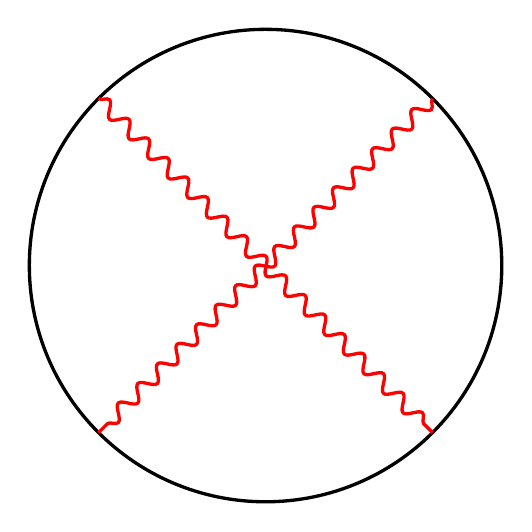
\begin{tikzpicture}[scale=2,>=stealth]
%Draw Circle radius 1 cm
  \def\radi{1.5cm}
    \draw[black,very thick] (0,0) circle (\radi);
   % \foreach \angle/\count in {45/1,135/2,225/3,315/4}
    %    {
        
\tikzset{snake it/.style={decorate, decoration=snake}}
%Draws the 3 acceleration vectors directed inward and offset slightly from the distance vectors
       % \draw [name=acceleration vectors,very thick, snake it]
        %    (\angle:1.2cm) -- node[midway] {} (\angle:0.9cm) ;
         %     \path [draw=blue,snake it](-4,0) -- (-2,0) -- (2,0) -- (4,0);
  %\draw[draw=blue, snake it] (2,0) arc (0:180:2cm);
   % } snake it
    
        \path[coordinate] (0,0)  coordinate(A)++( 45:\radi) coordinate(B1);
        \path[coordinate] (0,0)  coordinate(A)++( 135:\radi) coordinate(B2);
        \path[coordinate] (0,0)  coordinate(A)++( -45:\radi) coordinate(B3);
        \path[coordinate] (0,0)  coordinate(A)++( -135:\radi) coordinate(B4);
        \draw[draw=red, snake it, very thick] (B1)--(B4);
        \draw[draw=red, snake it, very thick] (B2)--(B3);
\end{tikzpicture}
\end{figure}
 \begin{align*}
  ds^2=\frac{1}{\cos^2\rho} \left( d \rho^2 + dt^2 + \sin^2 \rho \Omega^2_{d-1} \right)
 \end{align*}
  The K-G equation in global coordinates is given by (where $m^2=\Delta(\Delta-d)$):
  \begin{align}
   \left( \cos^2 \rho \partial^2_\rho + (d-1)\cot \rho \partial_\rho + \cos^2 \rho \partial^2_t -m^2 \right) \phi^{12}_{\Delta}(y) = 0 \label{KGglob}
  \end{align}
  Now, the time dependence of $\phi$ may be calculated by considering the product of two bulk-to-boundary propagators on a fixed time $t$ slice:
  \begin{align*}
   \mathcal{K}(t,t_1) \mathcal{K}(t,t_2) \propto e^{-\Delta_{12}t}
  \end{align*}
  plugging this into eqn. \ref{KGglob} gives
  \begin{align}
   \left( \cos^2 \rho \partial^2_\rho + (d-1)\cot \rho \partial_\rho + \cos^2 \rho \Delta_{12}^2 -m^2 \right) \phi^{12}_{\Delta}(y) = 0 \label{KGglob1}
  \end{align}
  
  This differential equation can be converted into the hypergeometric equation with the correct choice of substituitions. Changing the variables from $\rho \to \eta$ with the substituition $\eta = \cos ^2 \rho$ gives:
  \begin{align}
   \left( 2 \eta (\eta-1)  \partial_\eta^2 + (d-2+2 \eta) \partial_\eta + \frac{\eta \Delta_{12}^2 - \Delta(\Delta-d) }{2\eta} \right) \phi = 0
  \end{align}
  The further substitution $\phi(\eta) = \eta^{\Delta/2} f(\eta)$ (or $\phi(\eta) = \eta^{(d-\Delta)/2} f(\eta)$) reduces the equation to a hypergeometric equation:
    \begin{align}
   \left[ \eta (1-\eta)  \partial_\eta^2 + \left(-\frac{d}{2}+1+\Delta -(1+\Delta)\eta\right) \partial_\eta - \frac{\Delta^2-\Delta_{12}^2}{4} \right] f(\eta) = 0
  \end{align}
  This has the same form as the hypergeometric differential equation
  
  \begin{align}
   z(1-z)\frac{d^2 w}{dz^2} + (c-(1+a+b)z)\frac{dw}{dz}-abw =0
  \end{align}
  for
  \begin{align}
   a &= \frac{\Delta-\Delta_{12}}{2} \\
   b &= \frac{\Delta+\Delta_{12}}{2} \\
   c &= -\frac{d}{2}+\Delta +1
  \end{align}
  Which gives the solution
  \begin{align}
   f(\eta) &= {}_2 F_1 \left(\frac{\Delta-\Delta_{12}}{2},\frac{\Delta+\Delta_{12}}{2},-\frac{d}{2}+\Delta +1; \eta \right) \\   
   \implies \phi^{12}_{\Delta}(\rho) &=  {}_2 F_1 \left(\frac{\Delta-\Delta_{12}}{2},\frac{\Delta+\Delta_{12}}{2} ,  -\frac{d}{2}+\Delta +1 ; \cos^2 \rho \right) \cos^\Delta \rho 
  \end{align}
  Then the full solution including time dependence is given by
 \begin{multline}
   \phi^{12}_{\Delta}(\rho, t) = \beta_{\Delta 1 2 } e^{\Delta_1 t_1 - \Delta_2 t_2}\times e^{-\Delta_{12}t} \\ \times {}_2 F_1 \left(\frac{\Delta-\Delta_{12}}{2},\frac{\Delta+\Delta_{12}}{2} ,  -\frac{d}{2}+\Delta +1 ; \cos^2 \rho \right) \cos^\Delta \rho
 \end{multline}
  Now, as we see from \ref{eqw} and \ref{eqphi} we need to evaluate $\phi^{12}_{\Delta}(\rho, t)$ on the geodesic $\gamma_{34}$. This is most conveniently done in Poincar\'{e} coordinates since in Poincar\'{e} AdS$_3$ the geodesics are just semi-circles. However, the transformation properties of the function $\phi^{12}_{\Delta}$ are not trivial when moving from global to Poincar\'{e} coordinates. The bulk-bulk propagator $\mathcal{G}$ is a function of only the geodesic distance between the two boundary points, therefore independent of the 
  
  However, the bulk-to-boundary propagator is a solution of the homogenous AdS wave equation which diverges in a prescribed manner in the bulk.
  
  \begin{align}
   (\Box - m^2) \mathcal{K} = 0
  \end{align}
In Poincar\'{e} coordinates, the $u \to 0$ behavior of $\mathcal{K}$ is 
\begin{align}
 \lim_{u \to 0} \mathcal{K}_{Poincar\'{e}}(u,x;x^\prime) \to u^{\Delta_-}\delta(x-x^\prime)
\end{align}
This is because the non-renormalizable bulk modes of the AdS wave equation in Poincar\'{e} coordinates behave as $u^{\Delta_-}$ near the boundary and therefore $\mathcal{K}$ should reproduce that behavior when a source function on the boundary sources a bulk field.

However, the non-renormalizable bulk modes of the AdS wave equation in global coordinates behave as $\cos^{\Delta_-} \rho$ near the boundary. So 
\begin{align}
 \lim_{\rho \to \pi/2} \mathcal{K}_{global}(\rho,t,\Omega;t^\prime, \Omega^\prime) \to \cos^{\Delta_-}\rho \delta(x-x^\prime)
\end{align}
  check McGreevy http://physics.ucsd.edu/~mcgreevy/fall08/handouts/lecture14.pdf 
  
  The map from global coordinates $(\rho, t)$ to Ponicar\'{e} coordinates $u,x^i$ is given by
  \begin{align}
   e^{-2t} = u^2 + |x|^2, \;\;\;\; \cos^2\rho = \frac{u^2}{u^2 + |x|^2} \label{globaltopoincare}
  \end{align}

  Hence, the global and poincare bulk-to-boundary propagators differ by a factor of $|x_i|^{\Delta_i}$. Stripping these factors off, for the sake of convinience gives the function $\phi^{12}_{\Delta}$ in Poincare coordinates
   \begin{multline}
   \phi^{12}_{\Delta}(u,x^i) = \beta_{\Delta 1 2 } e^{\Delta_1 t_1 - \Delta_2 t_2}\times e^{-\Delta_{12}t} \\ \times {}_2 F_1 \left(\frac{\Delta-\Delta_{12}}{2},\frac{\Delta+\Delta_{12}}{2} ,  -\frac{d}{2}+\Delta +1 ; \cos^2 \rho \right) \cos^\Delta \rho \label{phipoincare}
 \end{multline}
 Where now the global coordinates $(\rho,t)$ on the right hand side of \ref{phipoincare} are to be viewed as functions of the Poincar\'{e} coordinates by \ref{globaltopoincare}. 
 
 Geodesics in AdS$_3$ are semi-circles, see appendex entry \ref{adsgeodesic}  for a derivation, and with the particular choice of coordinates in \ref{partialwave} the geodesic $\gamma_{34}$ connecting points $z_3 = 1-z$ and $z_4 = 1$ lies exactly in an AdS$_3$ slice of AdS$_{d+1}$. Therefore the equation of $\gamma_{34}$ can be written as 
 \begin{align}
  u^2 + 
 \end{align}

  \section{Mellin Space Representations of CFT Correlators}
  \subsection{Single Trace, double trace operators and shadow operators, conglomeration of operators}
  See fitzpatrick, kaplan, Unitarity and the Holographic S matrix
  \section{Monodromy Method}
  \section{Embedding Formalism and The Conformal Casimir}

%  \chapter{Conformal Blocks and the Semi-Classical Limit}

  \section{Introduction}
  \section{Spectrum of Semi-Classical Limits}
  \subsection{Global Limit}
  \subsection{Heavy-Light Limit}
  \subsection{Perturbative Heavy Limit}
  \subsection{Non-Perturbative Heavy Limit}
  \section{Operator Exchange: Spinless vs Spinning}
  %\subsection{Mellin Space Technology}
  \section{Monodromy Method and Liouville Theory}
  \section{Holographic Computation}
%  \chapter{Conformal Blocks and the Semi-Classical Limit} \label{ch:semiclassical}
  
  In accord with Zamolodchikov's $c$-theorem \cite{Zamolodchikov:1986gt}, the central charge $c$ of a 2D CFT is related to the number of degrees of freedom of the theory. Therefor the large $c$ limit naturally satisfies one of the requirements for a CFT to have a nice classical(?) gravity description. 
  
  see http://arxiv.org/pdf/1502.07742.pdf for Introduction
  
  Belavin, Polyakov and Zamolodchikov [BPZ] discovered in their ground breaking work \cite{Belavin:1984vu} that Virasoro blocks of 4-point functions containing contributions from all elements in the conformal family of the exchanged operator are completely fixed by the operator dimensions and the central charge $c$ of the theory.
  \section{Introduction-the realm of large central charge}
   Even before the advent of the AdS/CFT correspondence, the relationship between 3D gravity in AdS space and 2D CFTs was explored by Brown and Henneaux \cite{Brown:1986nw}. Using the Hamiltonian formalism they obtained the relation between the central charge $c$ of the CFT living on the conformal boundary of the AdS space to the radius of curvature $l$ of the AdS space(G is Newton's constant in 3D gravity):
 
 \begin{align}
  c=\frac{3l}{2G} \label{central}
 \end{align}
Subsequently, this result was reproduce by Ba\~{n}ados using the Cherm-Simons formulation in 1994 \cite{Banados:1994tn} and Balasubramanian and Kraus using AdS/CFT in 1999 \cite{Balasubramanian:1999re}.
  
  In this chapter, we will work exclusively in 2D CFTs. The semi-calssical limit corresponds to taking the large central charge $c \to \infty$ limit. This limit turns out to be particularly interesting because the large central charge $c \gg 1$ limit corresponds to $l \gg l_p$ as is evident from \ref{central} where $l_p$ is the planck length. This is the weakly coupled limit for the gravity theory in the bulk and therefore we can perform a weak-coupling expansion in $l_p/l$ in the bulk and $1/c$ in the boundary theory. In addition, the $c \to \infty$ limit has been shown to calculate the R\'{e}nyi entropy for a subsystem in a theory described by a 2D CFT \cite{Hartman:2013mia}. In this limit, keeping all other parameters ($h_i$, the operator dimensions of external and exchanged operators in this limit) constant, the infinite dimensional Virasoro algebra reduces simply to the global algebra with generators $L_{-1}, L_0$ and $L_1$
  \begin{align*}
   [L_m,L_n] = (m-n)L_{m+n} + \frac{c}{12}m(m^2-1) \delta_{m,-n}
  \end{align*}
  
  Moreover, from the AdS/CFT correspondence the CFT stress-energy tensor $T(z,\bar{z})$ and creation oeprators $L_n$ for $n \leq -2$ create gravitons in the bulk field[EXPAND]. Due to the relation \cite{central} the central charge in the CFT determines the strength of the gravitational interaction in the bulk gravity theory. 
  \subsection{Central Charge}

  \section{Spectrum of Semi-Classical Limits}
  There are a number of different possibilities to be considered for the involved operator dimensions when taking the large central charge $c \gg 1$ limit for conformal blocks. We can have all the operator dimensionss $h_i$ and the exchanged operator dimension $h_p$ held fixed in the limit $c\to \infty$. Or on the other hand, we may have the operator dimensions scaling with the central charge, i.e. hold $h_i/c$ and $h_p/c$ fixed in the limit $c \to \infty$. As a middle ground we could also have some operator dimensions, say $h_1, h_2$ held fixed while others say $h_3, h_4$ scale with the central charge. In what follows, operator dimensions that scale with the central charge will be referred to as ``Heavy'' and operator dimensions that remain fixed in the limit $c \to \infty$ will be referred to as ``Light''.
  \subsection{Global Limit}
  
  The global limit corresponds to computing the conformal block with all light operators. In this limit the Virasoro blocks have a particularly simple structure and reduces to the conformal block due to the global conformal algebra spanned by $L_{\pm 1}$ and $L_0$ as in the case of $d \geq 3$ CFTs\cite{Fitzpatrick:2015zha}. The global block has the form of a hypergeometric function. Let's see how this works.
  
  
  
  \subsection{Heavy-Light Limit}
  
  The heavy-light limit corresponds to taking some operator dimensions $h_L$ fixed (the ``light'' operators) and some operator dimensions $h_H$ (the ``heavy'' operators) scaling as c in the large $c$ limit. In particular we will consider two heavy and two light operators, in the 4-point function:
  \begin{align}
   \Braket{\mathcal{O}_{L_1}\mathcal{O}_{L_2}\mathcal{O}_{H_1}\mathcal{O}_{H_2}} = \Braket{0|\mathcal{O}_{L_1}\mathcal{O}_{L_2}\mathcal{O}_{H_1}\mathcal{O}_{H_2}|0} 
  \end{align}
  Using commuttivity of operators inside the correlator, this can be written as 
   \begin{align}
   \Braket{0|\mathcal{O}_{H_1}\mathcal{O}_{L_1}\mathcal{O}_{L_2}\mathcal{O}_{H_2}|0} = \Braket{\mathcal{O}_{H_1}|\mathcal{O}_{L_1}\mathcal{O}_{L_2}|\mathcal{O}_{H_2}} 
  \end{align}
  
  And so in the AdS/CFT picture one associates this correlator with a BTZ black hole (or defect) created by the heavy operators and the light operators sourcing geodesics in this background. We review this computation in section \ref{sec:num1}
  \subsection{Perturbative Heavy Limit}
  \subsection{Non-Perturbative Heavy Limit}
  \section{Operator Exchange: Spinless vs Spinning}
  %\subsection{Mellin Space Technology}
  \section{Monodromy Method and Liouville Theory}
  
  The semi-classical limit and the monodromy method for calculation of the semi-classical conformal blocks comes from Liouville theory. This section closely follows the discussion in \cite{Harlow:2011ny} and \cite{Fitzpatrick:2014vua}. Liouville theory was in the past sutied by Polyakov in the study of non-critical string theory \cite{Polyakov:1981rd}. More recently relations of quantum Liouville theory to 
certain 4 dimensional superconformal field theories have been explored\cite{Alday:2009aq}.

Liouville theory is described by the action

\begin{align}
 S= \frac{1}{4b^2} \int \mathrm{d}^2x  \sqrt{g} \left( g^{\alpha \beta} \partial_\alpha \phi \partial_\beta \phi + 2(1+b^2) R \phi + 16\lambda e^\phi\right)
\end{align}
Where $R$ is the Ricci tensor for the metric $g_{\alpha\beta}$. The quantum Liouville theory is a 2D conformal field theory.  
  
  Correlators of degenerate primary fields in 2D CFTs satisfy a particular linear differential equation
  
  
  
  The Monodromy method is a powerful technique used to compute the semi-classical Virasoro blocks in certain limits. Recall that a 2D CFT 4 point function may be expanded in conformal blocks $\mathcal{F}$ as :
  \begin{align}
  \left\langle O_1(\infty) O_2(0) O_3(z,\bar{z}) O_4(1)\right\rangle = \sum a_p \mathcal{F}(z,h_i,h_p,c) \mathcal{F}(\bar{z},\bar{h}_i,\bar{h}_p,c)
  \end{align}
  where $a_p$ denotes the product of OPE coefficients
  \begin{align}
   a_p = c_{12}^p c_{34}^p
  \end{align}
  The Virasoro block $\mathcal{F}$ includes contributions from all the descendants due to exchange of a primary p. Although the general form of the virasoro blocks is unknown, in the semi-classical limit with $c \gg 1$ and with $h_p/c \text{ and } h_i/c$ fixed, there is much evidence that the Virasoro blocks exponentiate, although there exists no direct proof from the definition of Virasoro blocks as sum over descendants.
  
  \begin{align}
   \mathcal{F}(z,h_i,h_p,c) \approx \exp \left[-\frac{c}{6} f\left( \frac{h_i}{c}, \frac{h_p}{c}, z\right)\right]
  \end{align}
  There exists no known explicit results for $f$ but only expansions around $z=0$:
  \begin{align}
   \frac{c}{6} f\left( \frac{h_i}{c}, \frac{h_p}{c}, z\right) = (h_1 + h_2 - h_p) \log z - \frac{(h_p +h_2 - h_1)(h_p + h_3 - h_4)}{2h_p} z + \mathcal{O} (z^2)
  \end{align}
  However, $f$ might be calulated as the solution to the following second order differential equation with the prescribed mondromy:
  \begin{align}
   \frac{d^2 \psi(z)}{dz^2} + T(z)\psi(z) =0
  \end{align}
with
\begin{align}
 T(z) = \sum_i \left(\frac{h_i/c}{(z-z_i)^2} - \frac{c_i}{z-z_i} \right)
\end{align}
Here $z_i$ are the points at which operators $\mathcal{O}_i$ are inserted, i.e. $(z_1,z_2,z_3,z_4)= (\infty,0,z,1)$ and the $c_i$'s are known as accessory parameters. Three of the $c_i$ may be determined by requiring that the function $T(z)$ vanish as $z^{-4}$ as $z \to \infty$
  
  
  \section{Holographic Computation} \label{sec:num1}
%  \chapter{Applications}
  \section{R\'enyi Entropy}
  Consider a system $S$, written as a combination of two subsystems $A$ and $B=A^\complement$, i.e. $S=A \cup B$. Then the whole Hilbert space may be written as a direct product of the individual Hilbert spaces, i.e. $\mathcal{H}_S= \mathcal{H}_A \otimes \mathcal{H}_B$. Let $\rho$ be the density operator of the complete system $S$, then the reduced density operator of the subsystem $A$ is found by taking a partial trace over the complementary Hilbert space $\mathcal{H}_B$, $\rho_A = \text{Tr}_B[\rho]$. An observer having access to only the subsystem $A$ but not the whole system $S$ measures this reduced density operator $\rho_A$. This situation appears in a number of experimental/gedanken situations, for example while studying the black hole information paradox (see appendix \ref{infoparadox}) or in the case of Open Quantum Systems in Quantum Computation where the system of interest is open (coupled to the environment). In this case the Entanglement Entropy for the system $A$ is given by the von-Neumann entropy of A i.e. $S_A=-\text{Tr}[\rho_A \ln \rho_A]$. 
  
  In Information Theory the R\'{e}nyi entropy is a generalisation of the Shannon entropy, Hartley entropy, the collision entropy and the min-entropy. In Quantum Mechanical systems it is defined as 
  \begin{align}
   S^{(\alpha)} = \frac{1}{1-\alpha} \ln \text{Tr}[rho^\alpha] \label{renyi} 
  \end{align}
  The entanglement entropy(EE) may be calculated from the R\'{e}nyi entropy by taking the limit $\alpha \to 1$:
  \begin{align}
   S_{EE} = \lim_{\alpha \to 1}  S^{(\alpha)} \label{eentropy}
  \end{align}
  We are primarily 
  
  If in a quantum field theory once can represent the density operator $\rho$ as a path integral, it is also possible to write $\rho^n$ as a path integral for integer $n$, and then one can extend the result for general $n$ by analytic continuation. Thereafter, once can use \ref{renyi} and \ref{eentropy} to compute the entanglement entropy. This procedure generally goes under the name of the Replica trick \cite{Calabrese:2004eu}.
The semi-classical Virasoro blocks calculated in the last chapter can be immediately used to reproduce the two interval R\'{e}nyi entropy on the plane \cite{Perlmutter:2015iya}. 
  \section{Conformal Bootstrap}
  \section{Cluster Decomposition Principle}
%  \chapter{Conclusions and Discussion}
\begin{appendices}
\chapter{}
Consider the two point function. We must have 
\begin{align*}
 \left\langle \phi_1(x_1) \phi_2(x_2)\right\rangle = \left| \frac{\partial x^\prime}{\partial x}\right|_{x=x_1}^{\Delta_1/d} \left| \frac{\partial x^\prime}{\partial x}\right|_{x=x_2}^{\Delta_2/d} \left\langle \phi_1(x_1^\prime) \phi_2(x_2^\prime) \right\rangle
\end{align*}
Since the Poincar\'{e} group is a subgroup of the Conformal group, due to rotational and translational invariance the two point functon may only depend on $r_{12}=|x_1-x_2|$. denote $\Braket{\phi_1(x_1)\phi_2(x_2)} \equiv f(x_1,x_2) = f(|x_1-x_2|)=f(r_{12})$. 
Then under the rescaling $x_1, x_2 \to \lambda x_1, \lambda x_2$. $f^\prime \equiv {df}/{d\lambda}$
\begin{align*}
 f(r)=\lambda^{\Delta_1/d} \lambda^{\Delta_2/d} f(\lambda r) = \lambda^c  f(\lambda r) \\
 \implies c\frac{\lambda^c}{\lambda} f(\lambda r) + \lambda^c f^\prime(\lambda r) r =0 \\
 \text{set } r = 1 \\
 \implies \frac{c}{\lambda} f(\lambda) + f^\prime(\lambda ) = 0 \\
 \implies \int \frac{f^\prime(\lambda )}{f(\lambda)} = - \int \frac{c}{\lambda} \\
 \implies f(\lambda) \propto \lambda^{-c}
\end{align*}


\chapter{The Black Hole Information Paradox} \label{infoparadox}
Essentially the black hole information paradox arises from the fact that a quantum mechanical treatment of black holes leads to evolution of a pure initial state into a mixed state. For a pure state described by its desity matrix $\rho$, 
\begin{align}
 Tr[\rho^2] = 1
\end{align}

and using a unitary time evolution operator $U(t^\prime, t)$, 
\begin{align*}
  \rho \xrightarrow{U(t)} U \rho U^\dag
  \implies Tr[U \rho U^\dag U \rho U^\dag] = Tr[ U^\dag U \rho \rho] =  Tr[\rho^2] =1
 \end{align*}

However, consider a shell of mass $M$ in a pure state $\Ket{\psi}_M$ collapsing to form a black hole.

\begin{figure}[!h]
\centering
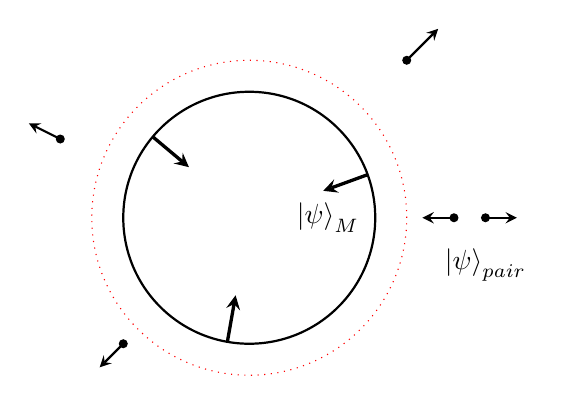
\begin{tikzpicture}[scale=2,>=stealth]
%Draw Circle radius 1 cm
    \draw[black,thick] (0,0) circle (0.8cm);
    \draw[red,dotted] (0,0) circle (1cm);
     \foreach \angle/\count in {20/1,140/2,260/3}
        {

%Draws the 3 acceleration vectors directed inward and offset slightly from the distance vectors
        \draw [name=acceleration vectors,very thick,->]
            (\angle:0.8cm) -- node[midway] {} (\angle:0.5cm) ;
    }
    \node[draw,circle,inner sep=1pt,fill] at (1,1)[] {};
    \node[draw,circle,inner sep=1pt,fill] at (1.5,0)[] {};
    \node[draw,circle,inner sep=1pt,fill] at (-1.2,0.5)[] {};
    \node[draw,circle,inner sep=1pt,fill] at (-0.8,-0.8)[] {};
    \draw [->,thick](1,1) -- (1.2,1.2);
    \draw [->,thick](1.5,0) -- (1.7,0);
    \draw [->,thick](-1.2,0.5) -- (-1.4,0.6);
    \draw [->,thick](-0.8,-0.8) -- (-0.95,-0.95);
    \node[draw=none] at (0.5,0) {$\Ket{\psi}_M$};
    
    \node[draw,circle,inner sep=1pt,fill] at (1.3,0)[] {};
    \draw [->,thick](1.3,0) -- (1.1,0);
    \node[draw=none] at (1.5,-0.3) {$\Ket{\psi}_{pair}$};
    
\end{tikzpicture}
\end{figure}

Due to the ``stretching'' of the spacelike slices, an entangled particle anti-particle pair in the sate given by:

\begin{align}
 \Ket{\psi}_\text{pair} \propto e^{\gamma c^\dag b^\dag} \Ket{0}_c \Ket{0}_b
\end{align}
Where c labels the infalling state and b labels the outgoing state. However, for qualitative purposes, it is enough to assume an entangled state of the form 
\begin{align}
 \Ket{\psi}_\text{pair} = \frac{1}{\sqrt{2}}(\Ket{0}_c \Ket{0}_b+\Ket{1}_c \Ket{1}_b)
\end{align}

The total state at this point is given (roughly) by

\begin{align}
 \Ket{\psi} \approx \Ket{\psi}_M \otimes \frac{1}{\sqrt{2}}(\Ket{0}_c \Ket{0}_b+\Ket{1}_c \Ket{1}_b)
\end{align}

and the entanglement entropy of the outgoing states (labeled by the subscript b) is given by a partial trace over the infalling state (labeled by subscript a) and the infalling mass shell M

\begin{align}
 S_b &= -Tr_{a,M}[\rho \log \rho] \\
 \implies S_b &= \log 2 
\end{align}

This $S_b$ is the entanglement (von-Neumann entropy) entropy of the subsystem b
Similarly, after propagating the timelike slice N times one ends up in the state 
\begin{align*}
 \Ket{\psi} \approx \Ket{\psi}_M &\otimes \frac{1}{\sqrt{2}}(\Ket{0}_{c1} \Ket{0}_{b1}+\Ket{1}_{c1} \Ket{1}_{b1}) \\
&\otimes \frac{1}{\sqrt{2}}(\Ket{0}_{c2} \Ket{0}_{b2}+\Ket{1}_{c2} \Ket{1}_{b2}) \\
\cdots
\end{align*}

Which gives for the entanglement entropy of the outgoing radiation
\begin{align}
 S_\text{entanglement} = N\log 2 \label{eentropy}
\end{align}

However, the outgoing radiation can be understood as thermal radiation due to the black hole radiatng away its mass. Or equivalently as the infalling particles with negative energy reducing the energy of the black hole. In either case, eventually, the black hole completely evaporates and the only remaining part is the radiated particles (system labeled by subscript b)


\begin{figure}[!h]
\centering
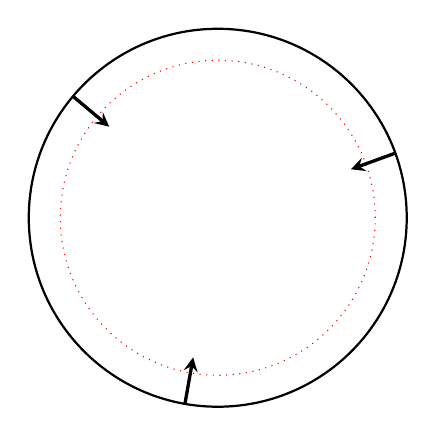
\begin{tikzpicture}[scale=2,>=stealth]
%Draw Circle radius 1 cm
    \draw[black,thick] (0,0) circle (1.2cm);
    \draw[red,dotted] (0,0) circle (1cm);
     \foreach \angle/\count in {20/1,140/2,260/3}
        {

%Draws the 3 acceleration vectors directed inward and offset slightly from the distance vectors
        \draw [name=acceleration vectors,very thick,->]
            (\angle:1.2cm) -- node[midway] {} (\angle:0.9cm) ;
    }
\end{tikzpicture}
\end{figure}



\begin{figure}[!h]
\centering
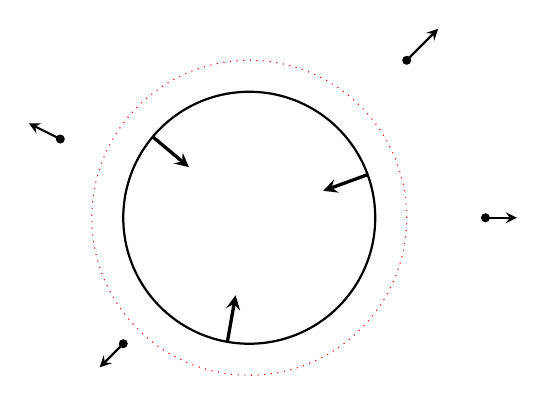
\begin{tikzpicture}[scale=2,>=stealth]
%Draw Circle radius 1 cm
    \draw[black,thick] (0,0) circle (0.8cm);
    \draw[red,dotted] (0,0) circle (1cm);
     \foreach \angle/\count in {20/1,140/2,260/3}
        {

%Draws the 3 acceleration vectors directed inward and offset slightly from the distance vectors
        \draw [name=acceleration vectors,very thick,->]
            (\angle:0.8cm) -- node[midway] {} (\angle:0.5cm) ;
    }
    \node[draw,circle,inner sep=1pt,fill] at (1,1)[] {};
    \node[draw,circle,inner sep=1pt,fill] at (1.5,0)[] {};
    \node[draw,circle,inner sep=1pt,fill] at (-1.2,0.5)[] {};
    \node[draw,circle,inner sep=1pt,fill] at (-0.8,-0.8)[] {};
    \draw [->,thick](1,1) -- (1.2,1.2);
    \draw [->,thick](1.5,0) -- (1.7,0);
    \draw [->,thick](-1.2,0.5) -- (-1.4,0.6);
    \draw [->,thick](-0.8,-0.8) -- (-0.95,-0.95);
\end{tikzpicture}
\end{figure}



\begin{figure}[!h]
\centering
\begin{tikzpicture}[scale=2,>=stealth]
%Draw Circle radius 1 cm
    \draw[black,thick] (0,0) circle (0.4cm);
    \draw[red,dotted] (0,0) circle (0.6cm);
     \foreach \angle/\count in {20/1,140/2,260/3}
        {

%Draws the 3 acceleration vectors directed inward and offset slightly from the distance vectors
        \draw [name=acceleration vectors,very thick,->]
            (\angle:0.4cm) -- node[midway] {} (\angle:0.2cm) ;
    }
    \node[draw,circle,inner sep=1pt,fill] at (1,1)[] {};
    \node[draw,circle,inner sep=1pt,fill] at (1.5,0)[] {};
    \node[draw,circle,inner sep=1pt,fill] at (-1.2,0.5)[] {};
    \node[draw,circle,inner sep=1pt,fill] at (-0.8,-0.8)[] {};
    \node[draw,circle,inner sep=1pt,fill] at (0,0.88)[] {};
    \node[draw,circle,inner sep=1pt,fill] at (0.6,-0.48)[] {};
    \draw [->,thick](1,1) -- (1.2,1.2);
    \draw [->,thick](1.5,0) -- (1.7,0);
    \draw [->,thick](-1.2,0.5) -- (-1.4,0.6);
    \draw [->,thick](-0.8,-0.8) -- (-0.95,-0.95);
    \draw [->,thick](0,0.88) -- (0,1.1);
    \draw [->,thick](0.6,-0.48) -- (0.7,-0.7);
\end{tikzpicture}
\end{figure}




\begin{figure}[!h]
\centering
\begin{tikzpicture}[scale=2,>=stealth]
%Draw Circle radius 1 cm
  
    \node[draw,circle,inner sep=1pt,fill] at (1,1)[] {};
    \node[draw,circle,inner sep=1pt,fill] at (1.5,0)[] {};
    \node[draw,circle,inner sep=1pt,fill] at (-1.2,0.5)[] {};
    \node[draw,circle,inner sep=1pt,fill] at (-0.8,-0.8)[] {};
    \node[draw,circle,inner sep=1pt,fill] at (0,0.88)[] {};
    \node[draw,circle,inner sep=1pt,fill] at (0.6,-0.48)[] {};
    \draw [->,thick](1,1) -- (1.2,1.2);
    \draw [->,thick](1.5,0) -- (1.7,0);
    \draw [->,thick](-1.2,0.5) -- (-1.4,0.6);
    \draw [->,thick](-0.8,-0.8) -- (-0.95,-0.95);
    \draw [->,thick](0,0.88) -- (0,1.1);
    \draw [->,thick](0.6,-0.48) -- (0.7,-0.7);
    
    \node[draw=none] at (0,0) {Poof!};
\end{tikzpicture}
\end{figure}


 
 
 Now, there is still a von-Neumann entropy associated with the system b given by \ref{eentropy} which is characterstic of a mixed quantum state since for a pure state we have $S=0$, and therefore to sum up, the system has evolved from a pure state to a mixed state which violates the unitarity of the time evolution operator. 

\chapter{Geometry of AdS$_{D+1}$}
\section{Global patch}
The global patch of AdS$_{D+1}$ is parametrised by the coordinates $(\rho,t, \Omega_D)$ where $\rho \in [0,\pi/2)$ is the radial coordinate (with the radial distance given by $\cos \rho$), $t \in (-\infty,\infty)$ is the time coordinate and $\Omega_{D-1}$ are the standard coordinates on the (D-1) dimensional sphere $S_{D-1}$. 

\begin{align}
 ds^2 = \frac{R^2}{\cos^2 \rho} \left( -dt^2 + d\rho^2 + \sin^2\rho d\Omega_{D-1}^2 \right) \label{globads}
\end{align}

\section{Poincar\'{e} patch}
The Poincar\'{e} patch of AdS$_{D+1}$ is parametrised by the coordinates $(u,x^0, x^1, \cdots x^D)$ (for $u \geq 0$, the upper half plane or UHP for short) where $u=0$ corresponds to the (conformal) boundary, and the metric is given by  

\begin{align}
 ds^2 = \frac{R^2}{u^2} \left( -dx_0^2 + du^2 + \sum_{i=1}^D dx_i^2 \right) \label{poincareads}
\end{align}


\section{Embedding Formalism}
Many calculations in AdS space are simplified by embedding AdS$_{D+1}$ in the D+2 flat space with metric
\begin{align}
 ds^2 = -dX_0^2 -dX_{D+1}^2+\sum_{i=1}^D dX_i^2
\end{align}
The AdS$_{D+1}$ space is then (the open cover of) the D+1 dimensional subspace defined by the equation
\begin{align}
 -X_0^2 -X_{D+1}^2+\sum_{i=1}^D X_i^2 = -R^2
\end{align}
or to be concise,
\begin{align}
 X^A X_A = -R^2 \label{embedads}
\end{align}


\section{Embedding Formalism(Euclidean)}
Many calculations in AdS space are simplified by embedding euclidean AdS$_{D+1}$ in the D+2 dimensional minkowski
\begin{align}
 ds^2 = -(dX^{-1})^2 +(dX^{0})^2+\sum_{i=1}^D (dX^i)^2
\end{align}

or introducing the light-cone coordinates $X^\pm = X^{-1} \pm X^0$,

\begin{align}
 ds^2 = -dX^+dX^-+\sum_{i=1}^D (dX^i)^2
\end{align}

The AdS$_{D+1}$ space is then (the open cover of) the D+1 dimensional subspace defined by the equation
\begin{align}
 -(X^{-1})^2 +(X^0)^2+\sum_{i=1}^D (X^i)^2 = -R^2
\end{align}
or to be concise,
\begin{align}
 X^A X_A = -R^2 \label{embedads}
\end{align}

The Poincar\'{e} coordinates on Euclidean AdS are then defined as 
\begin{align}
 X^+ = \frac{u^2 + |x|^2}{u}, \;\;\; Y^- = \frac{1}{u}, \;\;\; Y^i = \frac{x^i}{u}
\end{align}


In the embedding space, the infinitesimal generators of the group of Lorentz transformations in D+2 dimensions, SO(D+1,1) are 
\begin{align}
 L_{AB} = X_A \partial_B - X_B \partial_A
\end{align}
Moreover, the isometry group of euclidean AdS$_{D+1}$ is exactly SO(D+1,1), and so we can identify the generators $L_{AB}$ with the isometry generators of euclidean AdS$_{D+1}$
Then $L$ is a Casimir operator (an operator which commutes with all other operators in the algebra $[L,L_{AB}]=0$) with
\begin{align}
 L=\frac{1}{2} L_{AB}L^{AB} = \frac{1}{2}\left(X_A \partial_B - X_B \partial_A\right)\left(X^A \partial^B - X^B \partial^A\right)
\end{align}



Note that unlike Lorentzian AdS, in Euclidean AdS, the Poincar\'{e} coordinates cover the whole space, just like the global coordinates.

\section{Geodesics} \label{adsgeodesic}
One could calculate the geodesics in AdS$_{D+1}$ directly by extremising the following action
\begin{align}
 S= \int \mathrm{d} \lambda \; \sqrt{g_{\mu \nu} {\frac{dx^\mu}{d\lambda}} {\frac{dx^\nu}{d\lambda}} }
\end{align}
where for AdS$_{D+1}$ the metric $g_{\mu\nu}$ can be read off from \ref{globads} in global coordinates and \ref{poincareads} in Poincar\'{e} coordinates for the Poincare patch.

However, in practice this method gets fairly tedious and messy. Instead, it is customary to go to the embedding D+2 dimensional space and find the geodesics there subject to the contraint of equation \ref{embedads}. We shall work with the action [$(\cdot)^\prime = d(\cdot)/d\tau$]

\begin{align}
 S = \int {X^\prime}^A X^\prime_A + \lambda (X^A X_A + R^2 )
\end{align}

Where $\lambda$ is the lagrange multiplier. This gives the equations of motion
\begin{align}
 X_B^{\prime\prime} &= \lambda X_B \; \;\; B \in \{0,1,\cdots D+1 \} \\
 X^A X_A &= -R^2 
\end{align}
Let's focus on the first equation for now. Since the proper time $\tau$ is an unphysical coordinate and $\lambda$ is an arbitrary parameter, we can rescale $\tau \to \tau/\sqrt{|\lambda|}$. This gives for the first equation of motion:
\begin{align}
 X_B^{\prime\prime} = \frac{\lambda}{|\lambda|} X_B 
\end{align}
that is essentially we have 3 choices $\frac{\lambda}{|\lambda|} = -1, 0, 1$ and these exactly correspond to timelike, null and spacelike geodesics.

In particular, in Euclidean AdS$_3$ geodesics are semi-circles starting and ending on the boundary. Euclidean AdS$_3$ may be parametrised with the Poincar\'{e} coordinates $(u,x,y)$ with the metric
\begin{align}
 ds^2 = \frac{du^2 + dx^2 + dy^2}{u^2} 
\end{align}

The geodesic between two points on the boundary $(x_1,y_1)$ and $(x_2,y_2)$ may be parametrised with the coordinate $u$ and the length $\Delta l$ between two points may be written as 

\begin{align}
 \Delta l = \int \frac{du}{u} \sqrt{\dot{x}^2 + \dot{y}^2 +1}
\end{align}
where now $\dot x \equiv dx/du$. And so the geodesic equation can be derived using the Euler-Lagrange equations with $\mathcal{L} =  \sqrt{\dot{x}^2 + \dot{y}^2 +1}/{u}$. With some elementary algebra and integration, one ends up with the equation for a circle in the plane normal to the boundary $u=0$ and passing through the points $(x_1,y_1)$ and $(x_2,y_2)$. The semi-circular geodesic is uniquely defined by the fact that it meets the boundary $u=0$ perpendicularly. [Insert fig]



\subsection{Timelike geodesics}
The timelike geodesics are given by

\begin{align}
  X_B^{\prime\prime} = - X_B \label{timelike}
\end{align}
Subject to the constraint $ X^A X_A = -R^2$.
The eqn \ref{timelike} has the general solution:
\begin{align}
 X_B = c_B \cos\tau + d_B \sin \tau
\end{align}
Where $c_B, d_B$ are constant (no explicit $\tau$ dependence) vectors subject to constraints due to $ X^A X_A = -R^2$ :
\begin{align}
 &c_A d^A = 0 \\
 &c_A c^A = -R^2 = d_A d^A 
\end{align}

A common approach is to parametrise the timelike (massive) geodesic in AdS with the global coordinates $(\rho, t, \Omega_{D-1})$. Identify $\tau \equiv t$, and then parametrise $c_A, d_A$ in terms of $\rho, \Omega_{D-1}$. The simplest solution is limiting to constant $\Omega_{D-1}$, choose 
\begin{align}
 &c^0=R=d^{D+1} \\
 &c^A=0=d^B \;:otherwise
\end{align}
This gives
\begin{align}
 &X^0 = R\cos t \\
 &X^{D+1} = R \sin t \\
 &X^A = 0 \; :otherwise
\end{align}

%\begin{figure}
 \centering
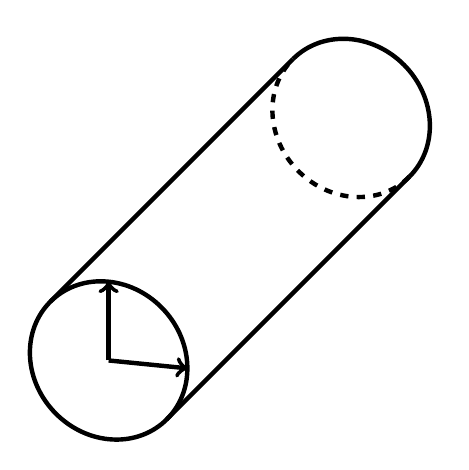
\begin{tikzpicture}

\begin{scope}[x={(1cm,-.1cm)}]
\path (1,0,0);
\pgfgetlastxy{\cylxx}{\cylxy}
\path (0,1,0);
\pgfgetlastxy{\cylyx}{\cylyy}
\path (0,0,1);
\pgfgetlastxy{\cylzx}{\cylzy}
\pgfmathsetmacro{\cylt}{(\cylzy * \cylyx - \cylzx * \cylyy)/ (\cylzy * \cylxx - \cylzx * \cylxy)}
\pgfmathsetmacro{\ang}{atan(\cylt)}
\pgfmathsetmacro{\ct}{1/sqrt(1 + (\cylt)^2)}
\pgfmathsetmacro{\st}{\cylt * \ct}
%\fill[red] (\ct,\st,0) -- ++(0,0,-8) arc[start angle=\ang,delta angle=180,radius=1] -- ++(0,0,8) arc[start angle=\ang+180,delta angle=-180,radius=1];
\begin{scope}[every path/.style={ultra thick}]
\draw (0,0,0) circle[radius=1];
\draw[->] (0,0,0) -- (1,0,0);
\draw[->] (0,0,0) -- (0,1,0);
\draw (\ct,\st,0) -- ++(0,0,-8);
\draw (-\ct,-\st,0) -- ++(0,0,-8);
\draw (\ct,\st,-8) arc[start angle=\ang,delta angle=180,radius=1];
\draw[dashed] (\ct,\st,-8) arc[start angle=\ang,delta angle=-180,radius=1];
\end{scope}
\end{scope}
\end{tikzpicture}
\end{figure}

\subsection{Null geodesics}
The null geodesic equation $ X_B^{\prime\prime} = 0$ has the general solution
\begin{align}
 X_B = c_B \tau + d_B
\end{align}
Along with the constrain equation $X^A X_A = -R^2$ this gives
\begin{align}
 &c_Ac^A = 0 = c_Ad^A \\
 &d_Ad^A=-R^2
\end{align}


\chapter{Differential Forms} \label{infoparadox}
Differential forms are a coordinate independent approach to multivariable calculus. They're specially useful in defining integrands over general manifolds without reference to a particular coordinate basis. Differential forms find many uses in physics and mathematics and are particularly useful when studying the \textbf{topological} properties of the manifolds. In particular, differential forms appear in the study of D-branes in string theory. D$p$-branes are dynamical objects in string theory charged under Raymond-Raymond p-forms. The general \emph{Stokes' Theorem} for Differential forms codifies a generalisation of the fundamental theorem of calculus, Greens' Theorem and Stokes' Theorem of multivariable calculus.


For a thorough discussion of differential forms and their various applications, refer to \emph{The Geometry of Physics} by Theodore Frankel \cite{frankel2004geometry}. The conventions used here are of that text.

Consider a finite dimensional(CHeck infinite?) vecotr space $E$, and its dual space $E^*$.  
\begin{definition}{\emph{Differential Form}}
A differential form of order p or a \textbf{p-form} $\omega_p$ is a totally antisymmetric tensor of rank $(0,p)$ ( a covariant $p$-tensor) $\omega_p \in \otimes^p E^*$:
\begin{align}
 \omega_p(\cdots,\bm{v}_r,\cdots,\bm{v}_s,\cdots) = -\omega_p(\cdots,\bm{v}_s,\cdots,\bm{v}_r,\cdots)
\end{align}
in each entry. Here $\bm{v}_m \in E \; \forall \; 1 \leq m \leq p$ 
\end{definition}

The collection of all $p$-forms forms a vector space which is a subspace of $\otimes^p E^*$, the tensor product space of p copies of the dual vector space $E^*$:
\begin{align}
 \bigwedge^p E^* = E* \wedge E^* \wedge \cdots \wedge E^* \subset  \otimes^p E^*
\end{align}

\begin{definition}{\emph{Wedge Product}}
A \textbf{wedge} or \textbf{exterior} or \textbf{Grassmann} product of a $p$-form and a $q$-form is a $p+q$-form: 
\begin{align}
 \wedge : \bigwedge^p E^* \times \bigwedge^q E^* \to \bigwedge^{p+q}E^*
\end{align}

for a $p$-form $\omega_p$ and a $q$-form $\eta_q$ 

in each entry. Here $\bm{v}_m \in E \; \forall \; 1 \leq m \leq p$ 
\end{definition}
\chapter{Hypergeometric Functions Toolbox} \label{hyper}
Hypergeometric functions 

This section closely follows Appendix B in \cite{Harlow:2011ny}.
\section{Hypergeometric series}
Consider the following series:
\begin{align}
 F(a,b;c,z) = \sum_{n=0}^\infty \frac{(a)_n(b)_n}{(c)_n n!} z^n
\end{align}
\section{Hypergeometric Differential Equation}

\section{Riemann's Differential Equation}
\end{appendices}
\bibliography{thesis}
\bibliographystyle{siam}
\end{document}
